% ==============================================================================
% PG - Sophie Dilhon
% Capítulo 4 - Projeto Arquitetural e Implementação
% ==============================================================================
\chapter{Projeto Arquitetural e Implementação}
\label{chap-projeto}

\vitor{Não iniciar um capítulo direto com uma seção ou uma seção direto com subseção. Adicionar um parágrafo explicando o que será apresentado neste capítulo, quando você tiver adicionado as demais seções.}

Após a definição dos requisitos, é necessário realizar o projeto arquitetural, nessa
fase as tecnologias utilizadas são incorporadas à modelagem do sistema. Neste capítulo
são apresentados os passos de planejamento e desenvolvimento da aplicação.
Na Seção~\ref{sec-projeto-tecnologias} estão as tecnologias utilizadas, na Seção~\ref{sec-projeto-frameweb}
são exemplificados os modelos FrameWeb desenvolvidos para auxilio na implementação do SCAP.
A Seção~\ref{sec-projeto-arquitetura} mostra a arquitetura do sistema. 
Por fim, na Seção~\ref{sec-projeto-impl} são apresentadas capturas de tela da aplicação para
ilustrar o desenvolvimento do SCAP.


\section{Tecnologias Utilizadas}
\label{sec-projeto-tecnologias}

Neste projeto, utilizou-se a linguagem \textit{TypeScript} unida ao \textit{framework} Next.js.
A Tabela~\ref{tab-tecnologias} apresenta as tecnologias e bibliotecas utilizadas, suas funções e suas respectivas versões.
Dentre as tecnologias, destaca-se o MySQL, um sistema de gerenciamento de banco de dados relacional,
e o Prisma, um ORM (\textit{Object-Relational Mapping}) para Node.js, ferramenta utilizada
para mapear classes para tabelas, além de facilitar a manipulação de dados com o banco.

\begin{table}[h]
    \centering
    \caption{Tecnologias e Bibliotecas Utilizadas.}
    \label{tab-tecnologias}
    \begin{tabularx}{\textwidth}{|p{4cm}|X|p{2cm}|}%{|p{3cm}|p{5cm}|p{5cm}|}
        \hline
        \textbf{Tecnologia} & \textbf{Função} & \textbf{Versão} \\
        \hline
        TypeScript & Linguagem de programação & 5 \\
        \hline
        Next.js & \textit{Framework} para desenvolvimento \textit{Web} & 14.1.3 \\
        \hline
        Tailwind CSS & \textit{Framework} CSS para estilizar componentes & 3.3.0 \\
        \hline
        Axios & Cliente HTTP baseado em \textit{Promises} & 1.6.8 \\
        \hline
        Prisma & ORM (\textit{Object-Relational Mapping}) para Node.js & 5.11.0 \\
        \hline
        MySQL & Sistema de Gerenciamento de Banco de Dados Relacional & 8.3.0 \\
        \hline
        React Dropzone & Componente para \textit{upload} de arquivos & 14.2.3 \\
        \hline
        React Input Mask & Componente para máscaras de \textit{inputs} & 3.0.0 \\
        \hline
        React Toastify & Componente para notificações & 10.0.5 \\
        \hline
        Luxon & Biblioteca para manipulação de datas & 3.4.4 \\
        \hline
        uuid & Biblioteca para geração de identificadores únicos & 9.0.1 \\
        \hline
        NPM & Gerenciador de pacotes para \textit{Node.js} & 10.5.0 \\
        \hline
        Visual Paradigm & Ferramenta para modelagem de diagramas & 17.1 \\
        \end{tabularx}
\end{table}




\section{Modelos FrameWeb}
\label{sec-projeto-frameweb}

Nessa seção são apresentados os modelos FrameWeb, construídos na fase de Projeto Arquitetural
do SCAP, com o objetivo de guiar a fase de implementação do sistema.

\subsection{Modelo de Entidades}
\label{subsec-frameweb-entidades}
O modelo de entidades de FrameWeb é um diagrama de classes UML que representam
os objetos de domínio do problema e seu mapeamento para a persistência no banco de dados
relacional. A partir dele são implementadas as classes da camada de domínio~\cite{souza:2007}.

A Figura~\ref{fig-modelo-entidades} apresenta o modelo de entidades do SCAP. O modelo foi feito
a partir do diagrama de classes mostrado anteriormente, com adaptações para a plataforma 
escolhida para a implementação do sistema, dessa forma são apresentados os tipos
de cada propriedade. A Figura~\ref{fig-modelo-entidades-enum} apresenta
os tipos enumerados do modelo de entidades do SCAP.

\begin{figure}
    \centering
    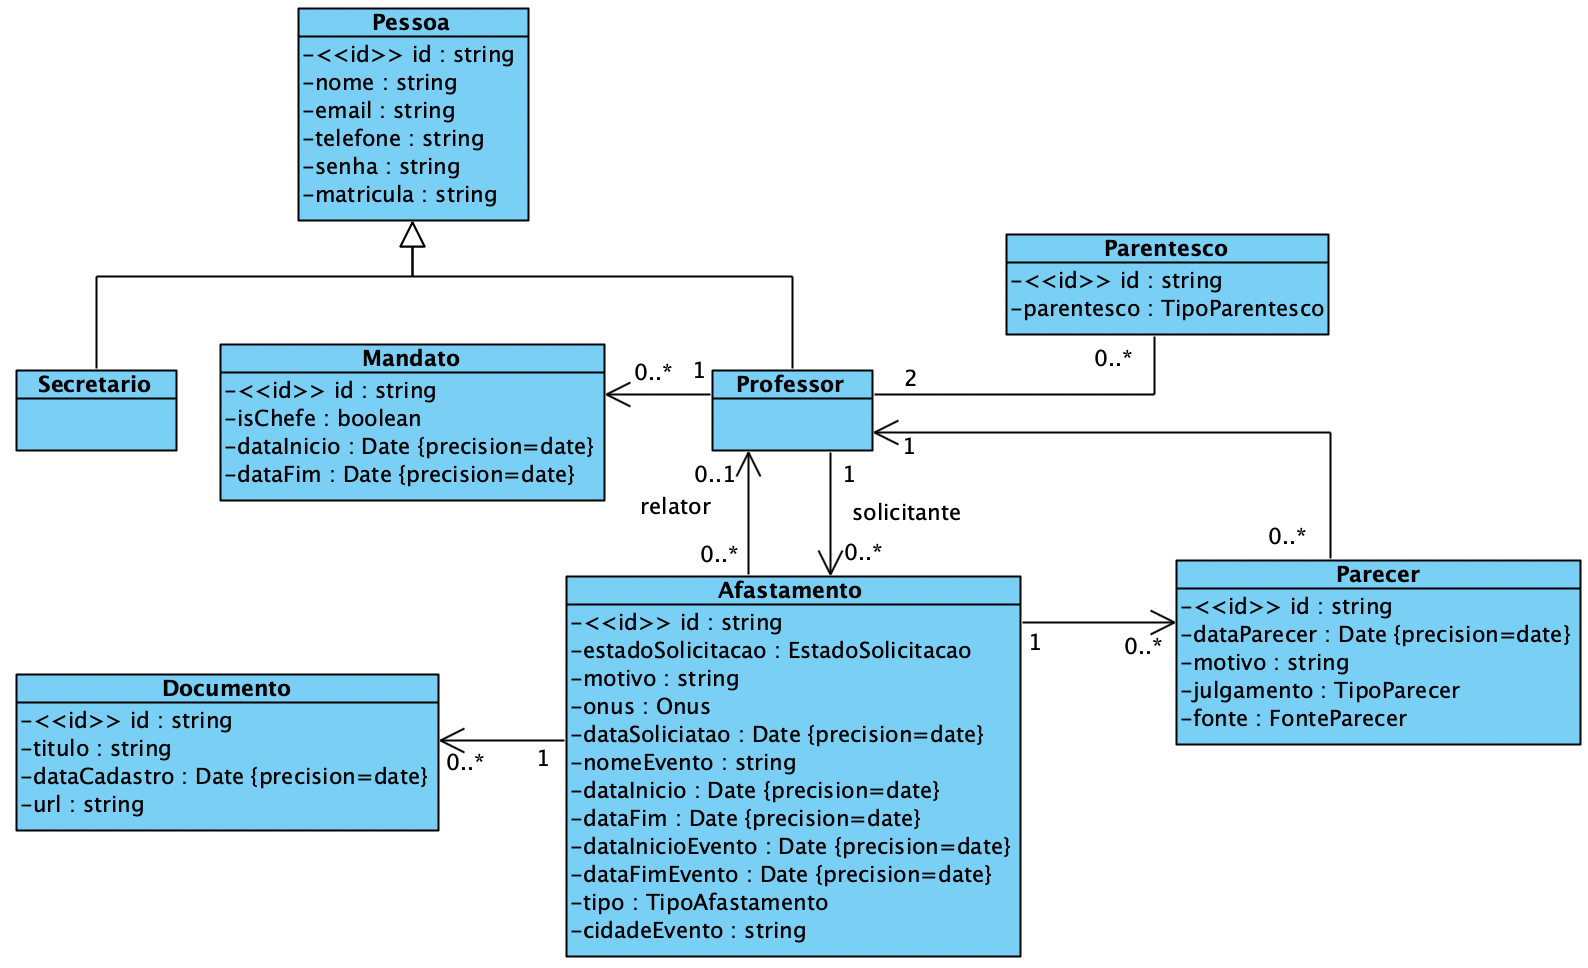
\includegraphics[width=1\textwidth]{figuras/fig-modelo-entidades.png}
    \caption{Modelo de Entidades do SCAP.}
    \label{fig-modelo-entidades}
\end{figure}

\vitor{Figura~\ref{fig-modelo-entidades}: 
	\begin{itemize}
		\item No TypeScript há um tipo de dado só pra datas e outro só pra horas ou existe apenas o \textsf{DateTime} usado no modelo? Se existir apenas um tipo unificado, é preciso especificar \textsf{precision=date} quando só estamos interessados na data (que é o caso na maioria das datas representadas no diagrama);
		\item As navegabilidades entre \textsf{Professor} e \textsf{Parentesco} foram pensadas pra ser desta forma mesmo? O objeto \textsf{p1} da classe \textsf{Professor} teria um atributo \textsf{parentesco} que se refere a uma instância da classe \textsf{Parentesco} que, por sua vez, tem um atributo \textsf{professor} que aponta para um objeto \textsf{p2} da classe \textsf{Professor}, mas \textsf{p2} não tem uma referência para este parentesco... Não seria melhor modelar como uma relação única \textsf{Professor} 2 -- 0.* \textsf{Parentesco}? A navegabilidade neste caso poderia ser dupla ou de \textsf{Parentesco} pra \textsf{Professor} apenas, pois essa informação é usada apenas num momento muito específico.
	\end{itemize}}

\sophie{Fiz as duas alterações}

\begin{figure}
    \centering
    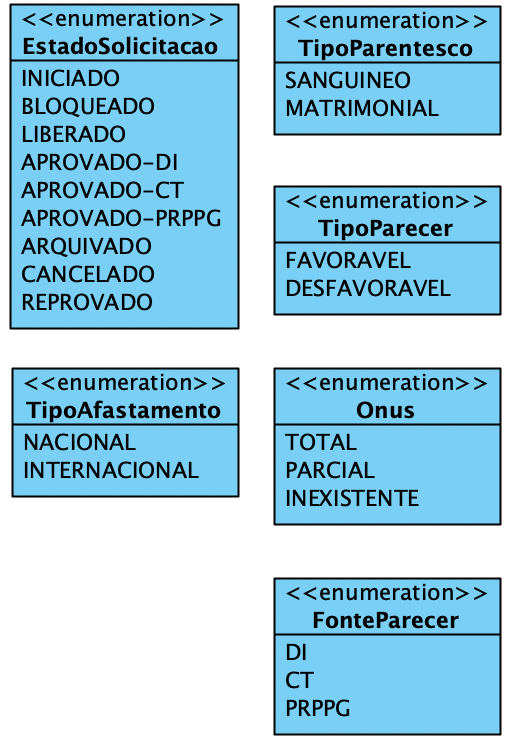
\includegraphics[width=0.5\textwidth]{figuras/fig-modelo-entidades-enum.png}
    \caption{Tipos Enumerados do Modelo de Entidades do SCAP.}
    \label{fig-modelo-entidades-enum}
\end{figure}


Os Diagramas~\ref{fig-diagrama-estado-nacional} e~\ref{fig-diagrama-estado-internacional} apresentam os fluxos de estados
para solicitações de afastamento do tipo nacional e internacional, respectivamente.
Explicitando os estados que uma solicitação de afastamento pode assumir e as transições entre eles,
de acordo com determinadas ações. Um exemplo de fluxo para um afastamento nacional é descrito abaixo:

\begin{enumerate}
    \item O professor solicita um afastamento nacional, este é criado no estado \textbf{INICIADO};
    \item Um professor do DI manifesta-se contra a solicitação, o afastamento passa para o estado \textbf{BLOQUEADO};
    \item Após votação favorável do colegiado, o secretário registra a aprovação do afastamento que muda para o estado \textbf{APROVADO\_DI};
    \item Por fim, o secretário arquiva a solicitação, modificando seu estado para \textbf{ARQUIVADO}.

\end{enumerate}

\begin{figure}[h!]
    \centering
    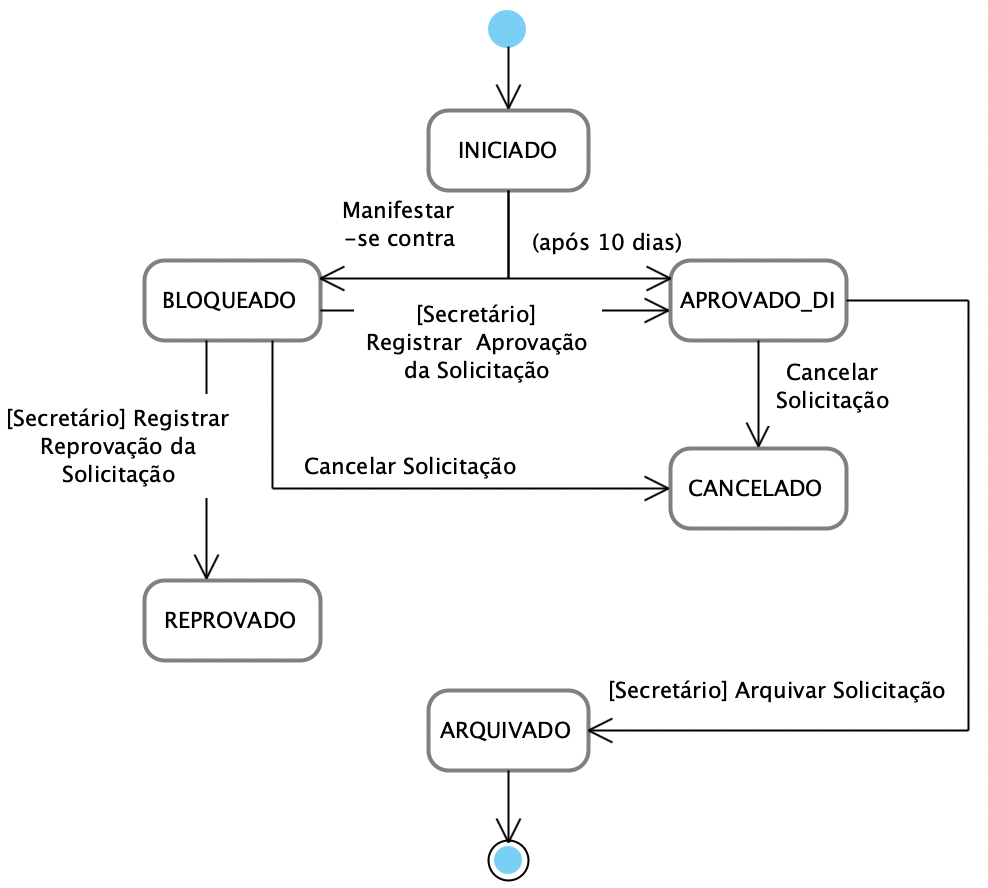
\includegraphics[width=0.8\textwidth]{figuras/fig-diagrama-estado-nacional.png}
    \caption{Diagrama de Estados da Solicitação de Afastamento Nacional do SCAP.}
    \label{fig-diagrama-estado-nacional}
\end{figure}


\begin{figure}[h!]
    \centering
    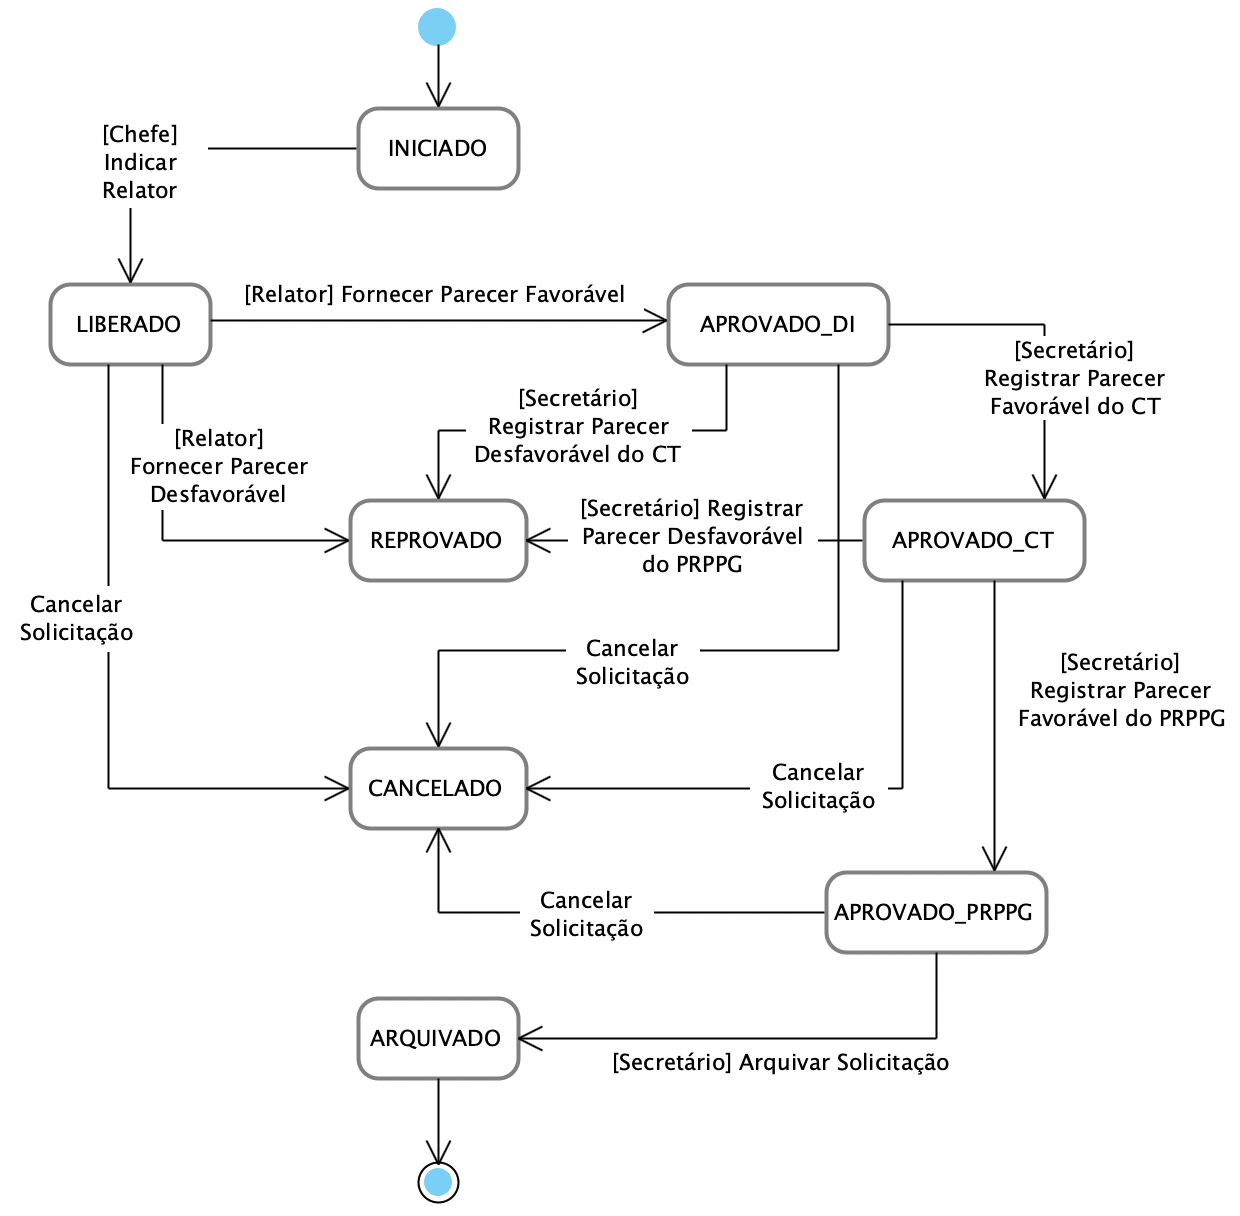
\includegraphics[width=0.9\textwidth]{figuras/fig-diagrama-estado-internacional.png}
    \caption{Diagrama de Estados da Solicitação de Afastamento Internacional do SCAP.}
    \label{fig-diagrama-estado-internacional}
\end{figure}


\subsection{Modelo de Persistência}
\label{subsec-frameweb-persistencia}

O modelo de persistência de FrameWeb é um diagrama de classes UML que representa
as classes responsáveis pela persistência das classes de domínio no banco de dados~\cite{souza:2007}.
Foi utilizado o padrão \textit{Repository} para a implementação das classes de persistência,
este propõe uma camada de separação entre o domínio e o mapeamento de dados.


Para isso, foi criada uma interface base (\textbf{IBaseRepositoy}) que define os métodos comuns a todas as classes de persistência,
sendo eles: \textit{get} para buscar todos os elementos com base nos filtros passados como parâmetro,
\textit{post} para criar um novo elemento, \textit{getById} para buscar um elemento a partir de seu
\textit{id} e \textit{delete}. A Figura~\ref{fig-modelo-persist-base} apresenta essa interface e a
classe \textit{Repository} que a implementa. O tipo genérico \textit{T} representa a classe de domínio
sendo manipulada, ou seja, em \textbf{AfastamentoRepository} o método \textit{getById}
retorna um elemento da classe \textbf{Afastamento}.


\begin{figure}[h!]
    \centering
    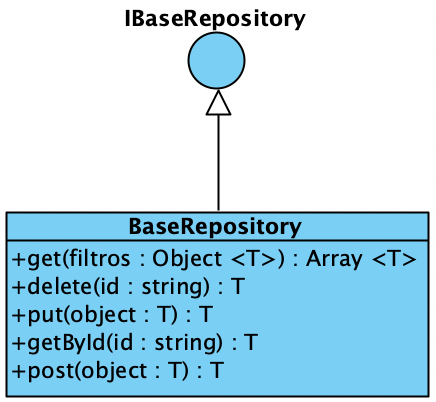
\includegraphics[width=0.4\textwidth]{figuras/fig-modelo-persist-base.png}
    \caption{Interface e Implementação do Repository Base.}
    \label{fig-modelo-persist-base}
\end{figure}


As interfaces do modelo herdam \textbf{IBaseRepositoy}, enquanto as classes \textit{Repository} estendem a
classe \textbf{BaseRepository}. De modo que todas as classes de persistência possuam, além dos métodos
específicos dessas, os métodos comuns definidos na interface base. As Figuras~\ref{fig-modelo-persist}
apresentam o modelo de persistência do SCAP.

\begin{figure}[h!]
    \centering
    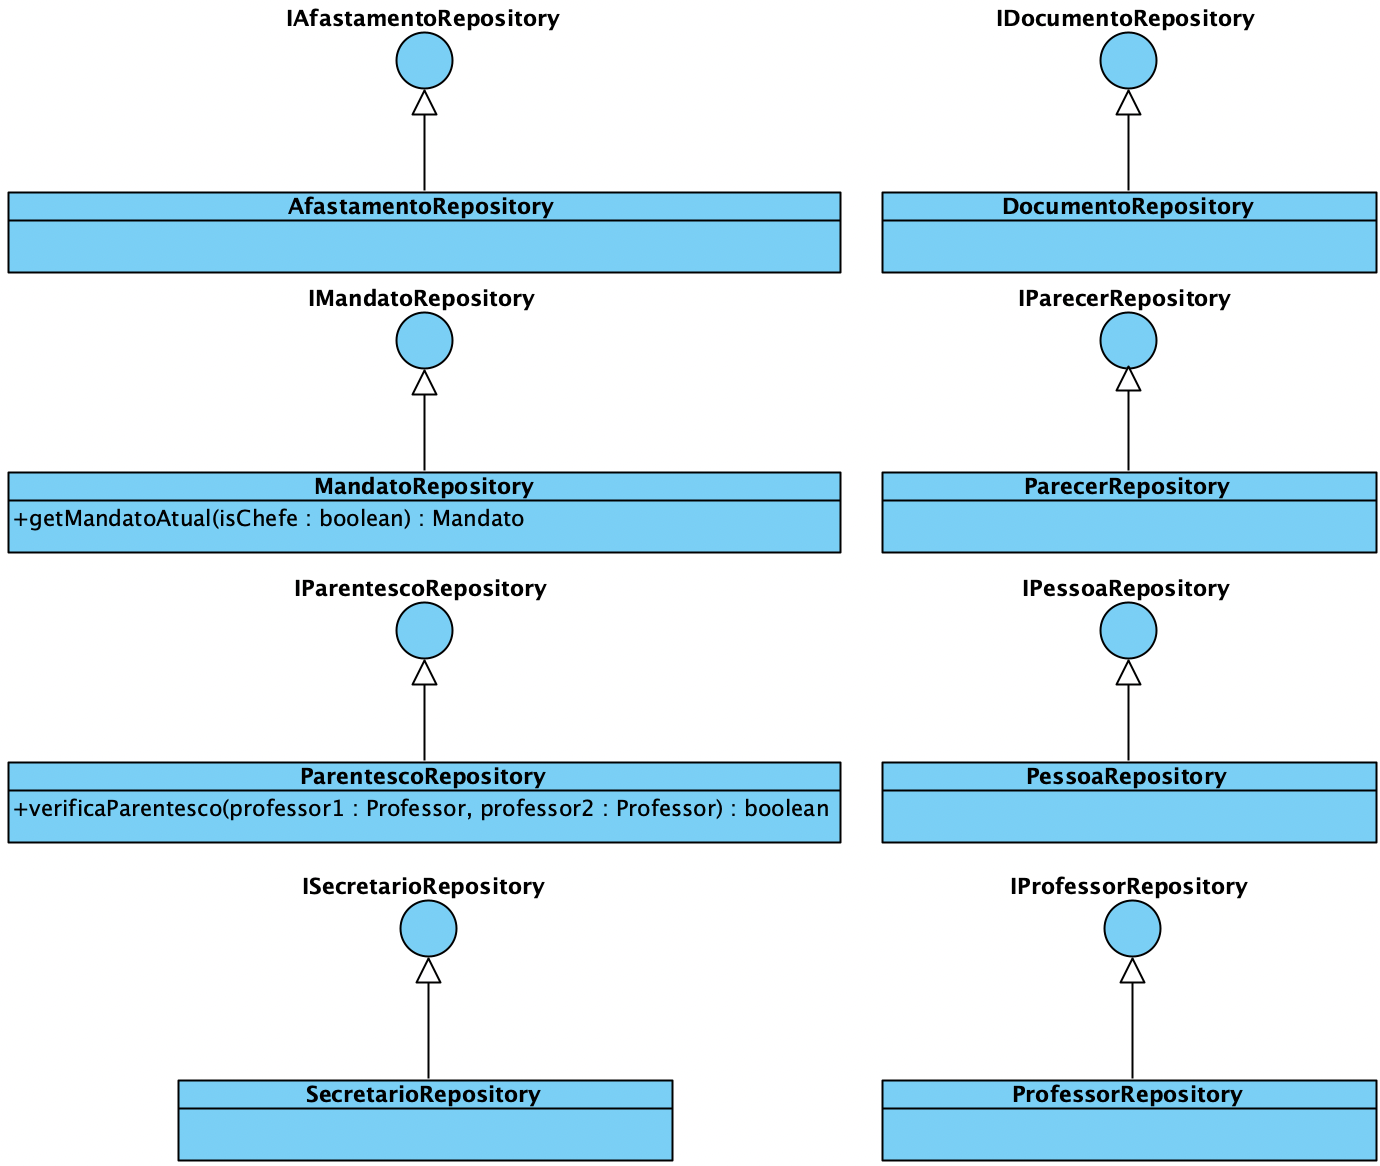
\includegraphics[width=0.9\textwidth]{figuras/fig-modelo-persist.png}
    \caption{Modelo de Persistência do SCAP.}
    \label{fig-modelo-persist}
\end{figure}

\vitor{Figura~\ref{fig-modelo-persist}: são só esses métodos mesmo que você precisou na implementação? Caso ainda vá avançar na implementação e surja a necessidade de novos métodos nos repositories, adicione-os neste modelo. 
	
	Além disso, o padrão de nome das interfaces é curioso. Eu imaginaria que a interface de \textsf{PessoaRepository} fosse \textsf{IPessoaRepository} e não apenas \textsf{IPessoa}. Esse é o padrão sugerido pelo \textit{framework} mesmo?}

\sophie{Só esses métodos foram usados mesmo.
    Sobre o padrão de nomes, pesquisando sobre o Repository Pattern vi que não existe um consenso em relação ao nome das interfaces e classes, mas achei que de fato ficou mais claro nomear as interfaces com o sufixo Repository.}

\subsection{Modelo de Navegação}
\label{subsec-frameweb-navegacao}

O Modelo de Navegação é um diagrama de classe da UML que representa os diferentes componentes que
formam a camada de Lógica de Apresentação, como páginas Web, formulários HTML e classes de ação do \textit{framework} específico~\cite{souza:2007}. 
Esse modelo é utilizado para guiar a implementação dos pacotes Visão e Controle.

A Tabela~\ref{tab-estereotipos-navegacao} apresenta os estereótipos UML utilizados no modelo de navegação do SCAP,
propostos por~\citeonline{hoppe:2023} como uma adaptação, para \textit{frameworks} SPA,
dos estereótipos propostos originalmente por~\citeonline{souza:2007}.

\begin{table}[h!]
    \centering
    \caption{Estereótipos UML para Modelos de Navegação~\cite{hoppe:2023}.}
    \label{tab-estereotipos-navegacao}
    \begin{tabular}{|p{3cm}|p{12cm}|}
        \hline
        \textbf{Estereótipo} & \textbf{Descrição} \\
        \hline
        (Nenhum)    & Controladora de um framework Front Controller ou a parte controladora de um component de um framework SPA. \\
        \hline
        <<Page>>    & Página Web estática ou dinâmica. \\
        \hline
        <<Partial>> & Parte de uma página HTML que é gerada em tempo de execução por meio de AJAX. \\
        \hline
        <<Form>>    & Formulário HTML \\
        \hline
    \end{tabular}
\end{table}

A Figura~\ref{fig-modelo-navegacao-afast} apresenta o modelo de navegação do SCAP para os casos de uso
\textbf{Cancelar Afastamento}, \textbf{Cadastrar Afastamento} e \textbf{Consultar Afastamento}.

\begin{figure}
    \centering
    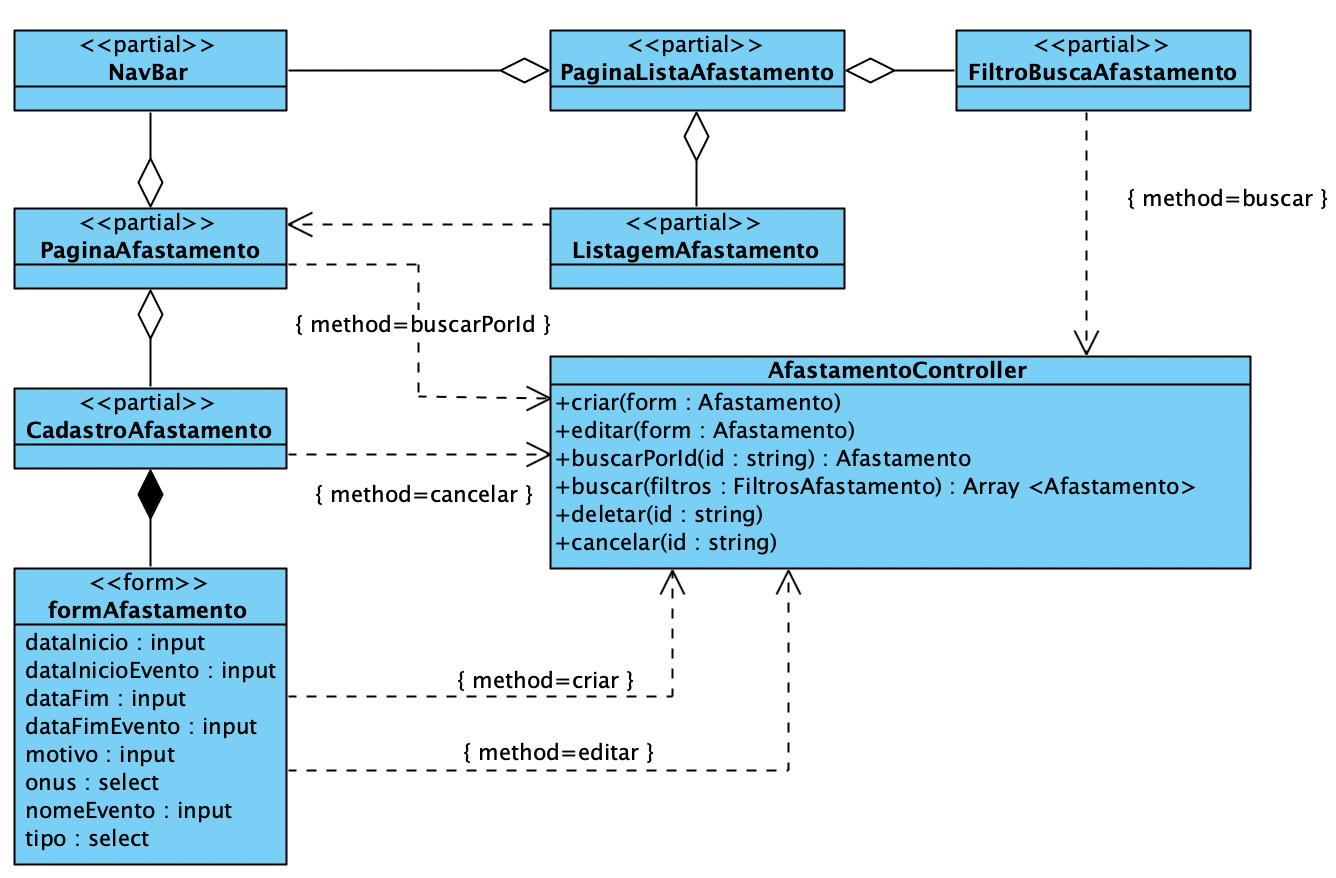
\includegraphics[width=1\textwidth]{figuras/fig-modelo-naveg-afast.png}
    \caption{Modelo de Navegação do SCAP.}
    \label{fig-modelo-navegacao-afast}
\end{figure}

A \textbf{PaginaListaAfastamento} é responsável por listar os afastamentos cadastrados.
Ela possui um componente filtro (\textbf{FiltroBuscaAfastamento}), em que é possível buscar
os afastamentos por diferentes critérios, definidos pela interface mostrada na Figura~\ref{fig-interface-filtro-afast}.
O componente \textbf{ListagemAfastamento} consiste de uma tabela que lista os afastamentos buscados,
cada linha da tabela possui um botão que redireciona para a página de detalhes do afastamento (\textbf{PaginaAfastamento}).

\begin{figure}
    \centering
    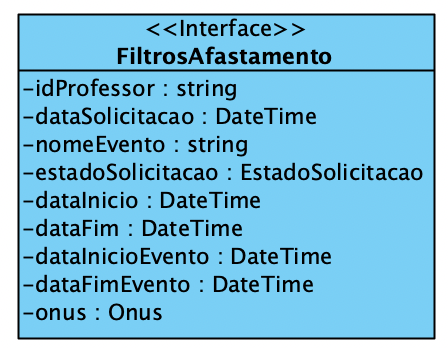
\includegraphics[width=0.4\textwidth]{figuras/fig-interface-filtro-afast.png}
    \caption{Interface Filtro Afastamento.}
    \label{fig-interface-filtro-afast}
\end{figure}

Se redirecionado para a \textbf{PaginaAfastamento} a partir do componente \textbf{ListagemAfastamento},
o \textit{partial} possui o atributo \textbf{id} inicializado com o \textit{id} do afastamento, e é
utilizado para fazer uma chamada ao método \textbf{buscarPorId} da \textit{controller} \textbf{AfastamentoController}.
Caso o usuário seja o solicitante do afastamento, ele pode cancelá-lo clicando em um botão que faz uma chamada ao método
\textbf{cancelar} da \textit{controller} \textbf{AfastamentoController}.

Quando não possui um \textit{id} inicializado, o \textit{partial} é utilizado para criar um novo afastamento,
o usuário deve então preencher os campos do formulário e clicar em um botão que faz uma chamada ao método
\textbf{criar} da \textit{controller} \textbf{AfastamentoController}.


\begin{figure}
    \centering
    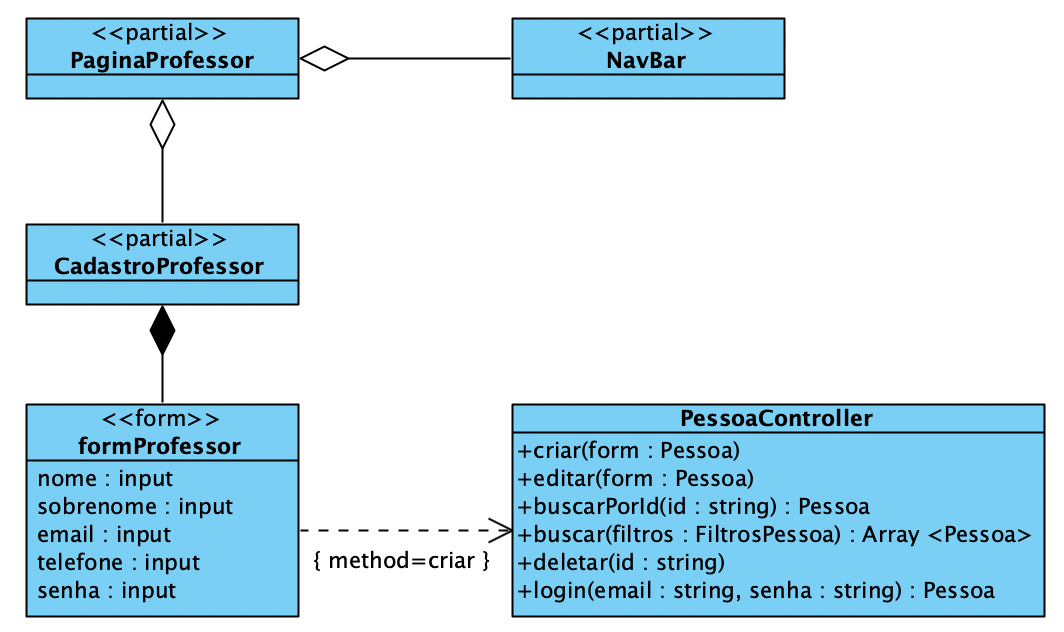
\includegraphics[width=0.9\textwidth]{figuras/fig-modelo-naveg-cadast.png}
    \caption{Modelo de Navegação do SCAP do Caso de Uso Cadastrar Professor.}
    \label{fig-modelo-navegacao-professor}
\end{figure}

A Figura~\ref{fig-modelo-navegacao-professor} apresenta o modelo de navegação do SCAP para o caso de uso
\textbf{Cadastrar Professor}. Na \textbf{PaginaProfessor} o secretário pode cadastrar um novo professor,
para isso ele deve preencher os campos do formulário e clicar em um botão que faz uma chamada ao método
\textbf{criar} da \textit{controller} \textbf{PessoaController}.

\vitor{Explicar o componente \textsf{NavBar} presente nas duas figuras.}

O componente \textbf{NavBar} presente em ambos os modelos de navegação é responsável por exibir
no topo da tela uma barra de navegação com links para as páginas principais do sistema, como a página inicial,
a página de listagem de afastamentos e a página de cadastro de professores. Ele é um componente
comum a todas as páginas do sistema, exceto à tela de \textit{login}.

\subsection{Modelo de Aplicação}
\label{subsec-frameweb-aplicacao}
O Modelo de Aplicação é um diagrama de classes da UML que representa as classes de
serviço, que são responsáveis pela codificação dos casos de uso, e suas dependências~\cite{souza:2007}.
Por ele pode-se visualizar a dependência entre os pacotes Controle (classes de ação),
Aplicação (classes de serviço) e Persistência (interfaces \textit{Repository}). 

As figuras~\ref{fig-modelo-aplicacao-1} e~\ref{fig-modelo-aplicacao-2} contém os Modelos de Aplicação.
As solicitações dos usuários são tratadas pelas classes de controle, que por sua vez
chamam as classes de serviço para realizar as operações de negócio, que por fim acessam
as classes de persistência para realizar as operações de leitura e escrita no banco de dados.


\begin{figure}[h!]
    \centering
    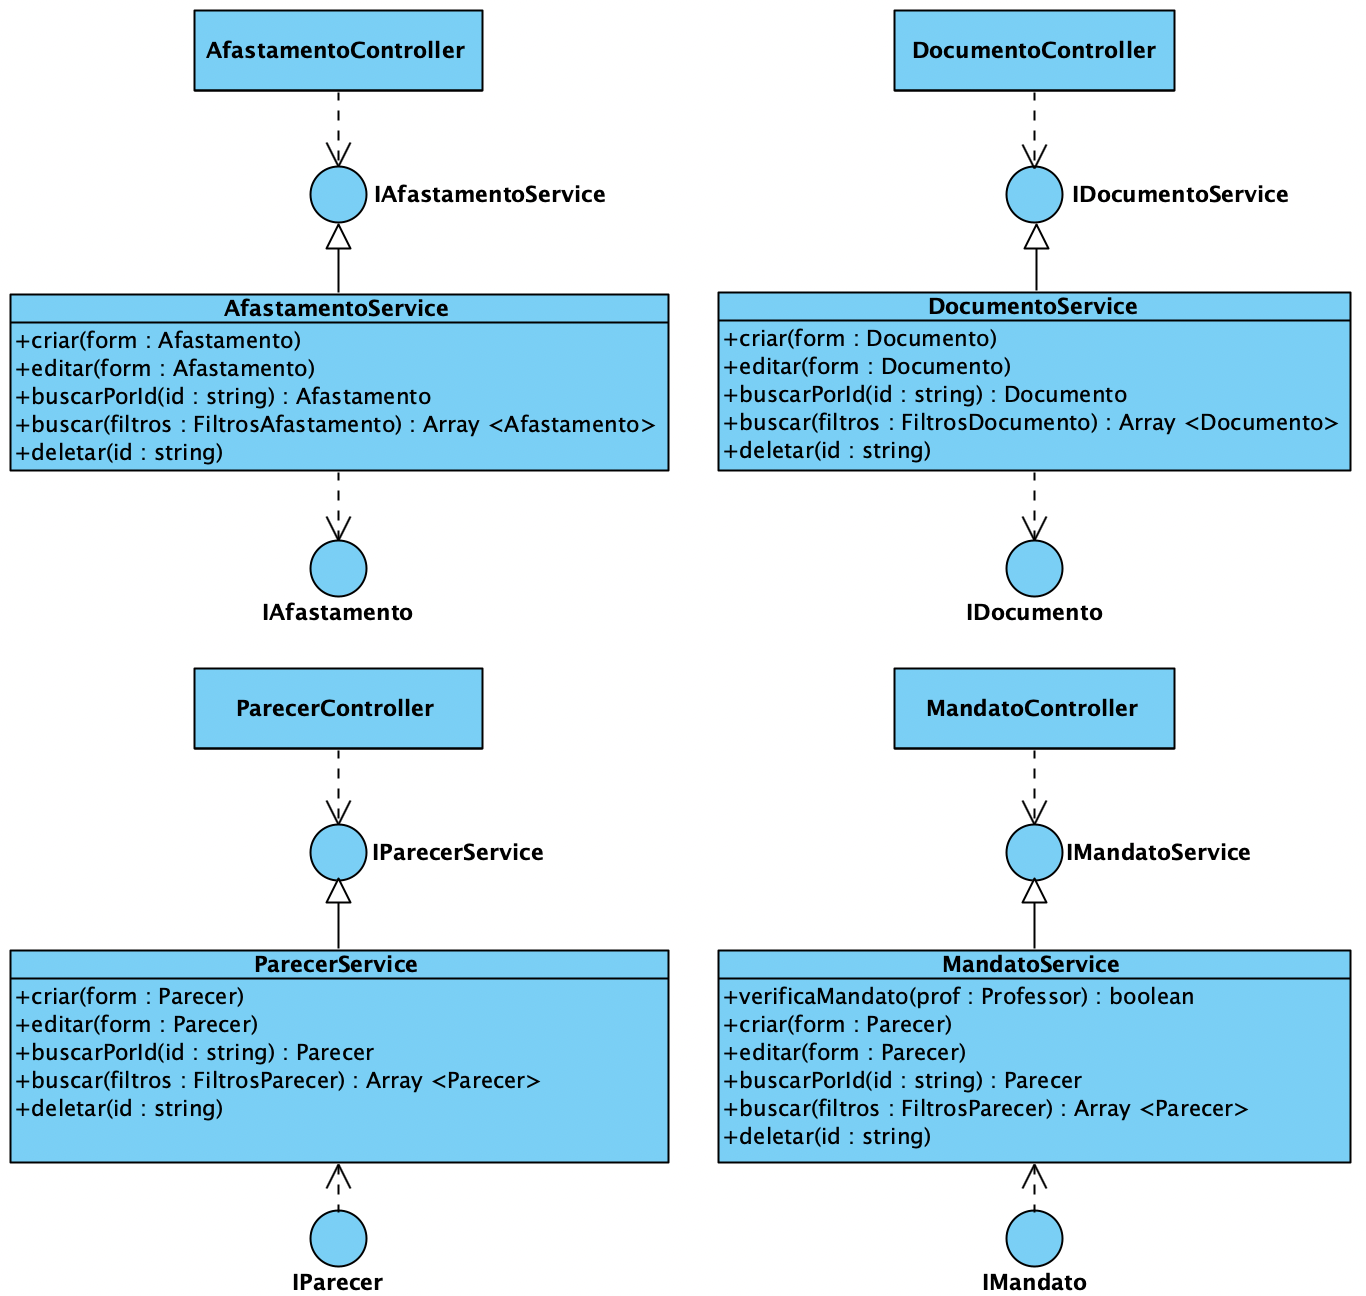
\includegraphics[width=0.9\textwidth]{figuras/fig-modelo-apl-1.png}
    \caption{Modelo de Aplicação do SCAP.}
    \label{fig-modelo-aplicacao-1}
\end{figure}

\vitor{Figura~\ref{fig-modelo-aplicacao-1}: acredito ue a direção da dependência entre \textsf{IParecer} e \textsf{ParecerService} esteja invertida, idem para \textsf{IMandato}. Além disso, foi usada uma relação de dependência entre as classes (controlador-serviço e serviço-repository). O FrameWeb geralmente usa uma associação entre essas classes, mas pode ser porque no Java, que é meu background, as classes de fato possuem um atributo que é uma referência pra outra classe. No seu caso uma dependência representa isso melhor? Se sim, inclua no texto uma explicação sobre isso.}
\sophie{Consertei as direções e verifiquei que a associação é mais adequada mesmo, então mudei para associação.}

\begin{figure}[h!]
    \centering
    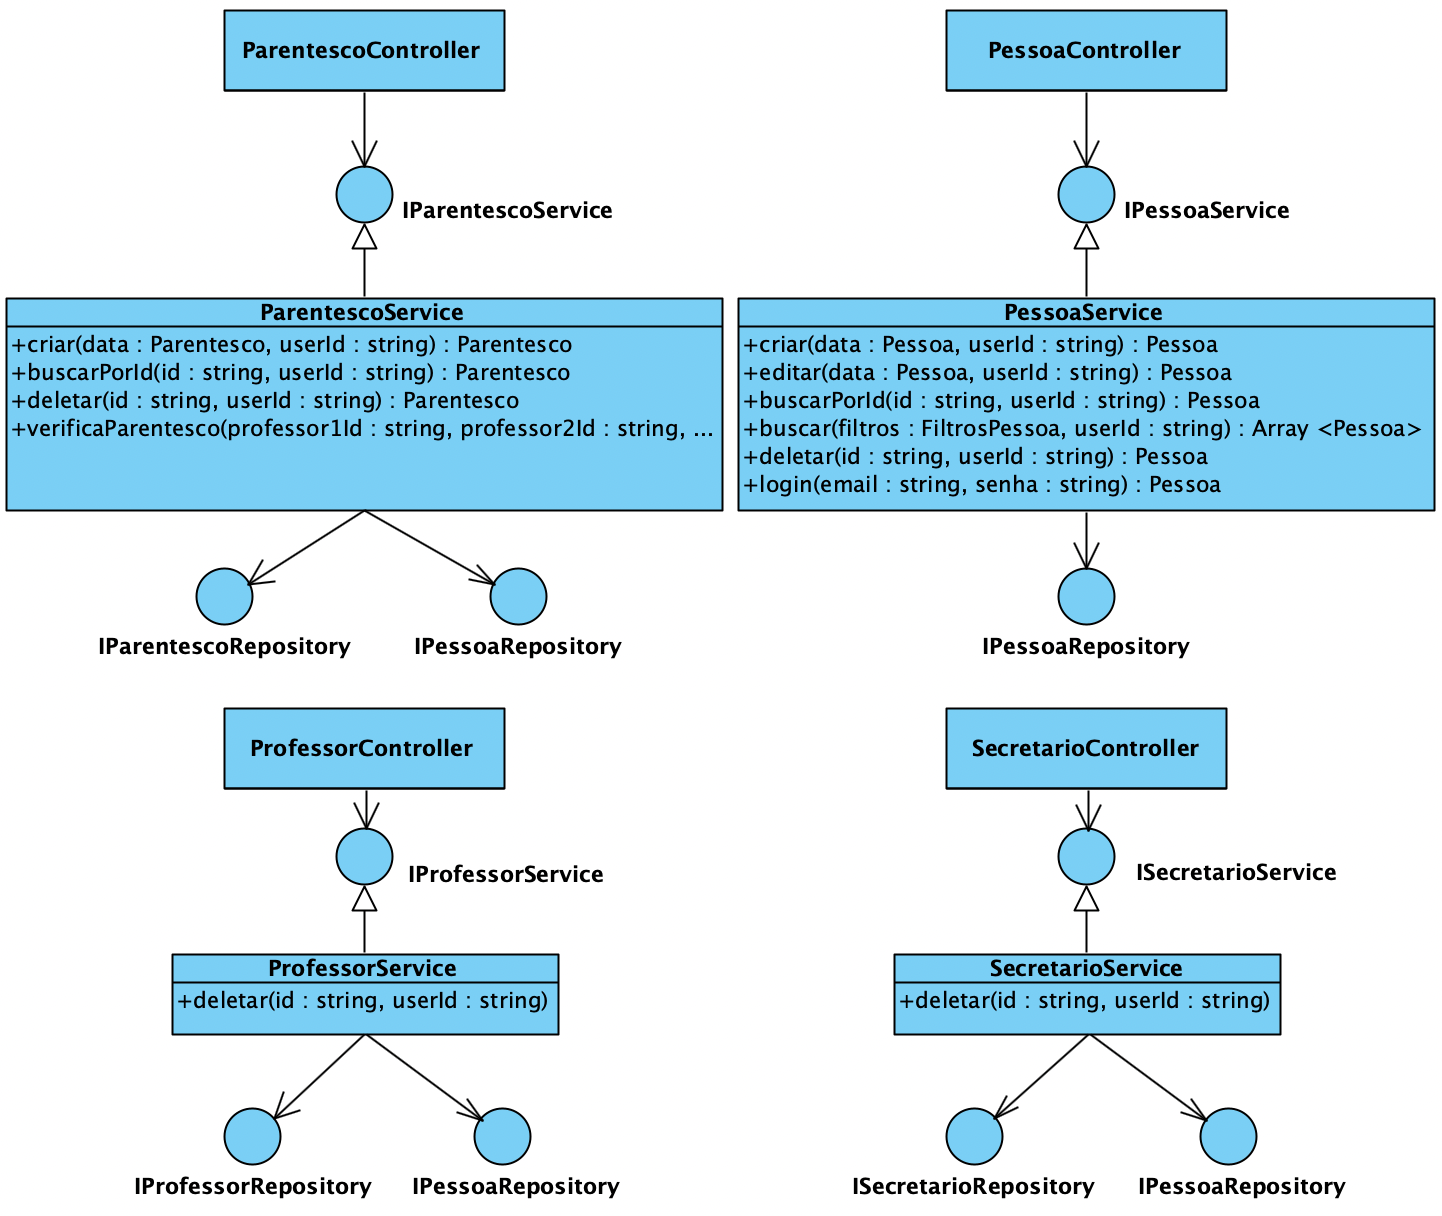
\includegraphics[width=0.9\textwidth]{figuras/fig-modelo-apl-2.png}
    \caption{Modelo de Aplicação do SCAP.}
    \label{fig-modelo-aplicacao-2}
\end{figure}



\section{Arquitetura do Sistema}
\label{sec-projeto-arquitetura}

Por ser um \textit{framework} de \textit{Single Page Application} (SPA), o Next.js funciona por meio de componentes,
e possui um padrão de \textit{design} diferente de projetos Java, por exemplo, que costumam utilizar
padrões como o \textit{Model-View-Controller} (MVC). 

A Figura~\ref{fig-pastas} apresenta a organização de pastas da implementação do SCAP. 
Na pasta \textbf{components} estão os componentes reutilizáveis, como o componente \textit{navbar} presente em todas as páginas do sistema.
A pasta \textbf{src} é a principal, nela estão contidas algumas pastas especiais controladas pelo \textit{framework}
como \textbf{pages} e \textbf{api}. A primeira, \textbf{pages}, transforma tudo que está dentro dela em uma rota do sistema,
ou seja, um arquivo \textit{index.js} em uma pasta chamada \textbf{pessoa} estará disponível como a rota \textit{/pessoa}.
De forma similar, a pasta \textbf{api} gera rotas de API a partir dos arquivos presentes nela.

Os arquivos presentes na pasta \textbf{api} possuem funções \textit{handler} especiais que são responsáveis por lidar com as requisições feitas ao servidor.
Estas funções utilizam as classes \textbf{controller} presente na pasta \textbf{lib} para manipular a requisição e retornar uma resposta.
Esta, por consequência, utiliza as classes \textbf{service} para realizar as operações de negócio, que por fim acessam as classes \textbf{reposity} para realizar
operações de leitura e escrita no banco de dados. As classes foram criadas seguindo o padrão de projeto \textit{Repository Pattern}.

No diretório \textbf{prisma} está presente o arquivo de configuração do Prisma, que contém o \textit{schema} do banco de dados e as \textit{migrations}
geradas pelo Prisma.

\begin{figure}
    \centering
    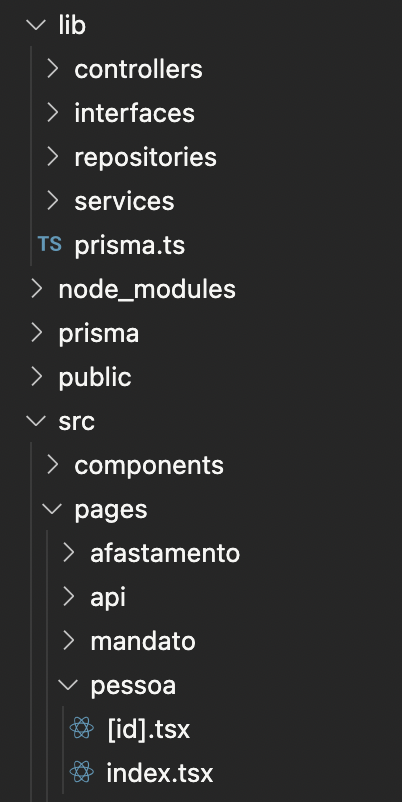
\includegraphics[width=0.4\textwidth]{figuras/fig-pastas.png}
    \caption{Arquitetura do SCAP.}
    \label{fig-pastas}
\end{figure}


\section{Implementação e Resultados}
\label{sec-projeto-impl}

Essa seção apresenta a implementação do SCAP, por meio de capturas de tela,
e discute os resultados obtidos.

\subsection{Login}
\label{subsec-projeto-login}

Para ter acesso ao SCAP, é necessário que o usuário realize o \textit{login} fornecendo o \textit{e-mail}
e senha cadastrados no sistema. A Figura~\ref{fig-login} apresenta a tela de \textit{login} do SCAP.
Por questões de segurança, sem o \textit{login} o usuário não consegue acessar as outras páginas do sistema
ou utilizar as rotas da API.

\begin{figure}[h!]
    \centering
    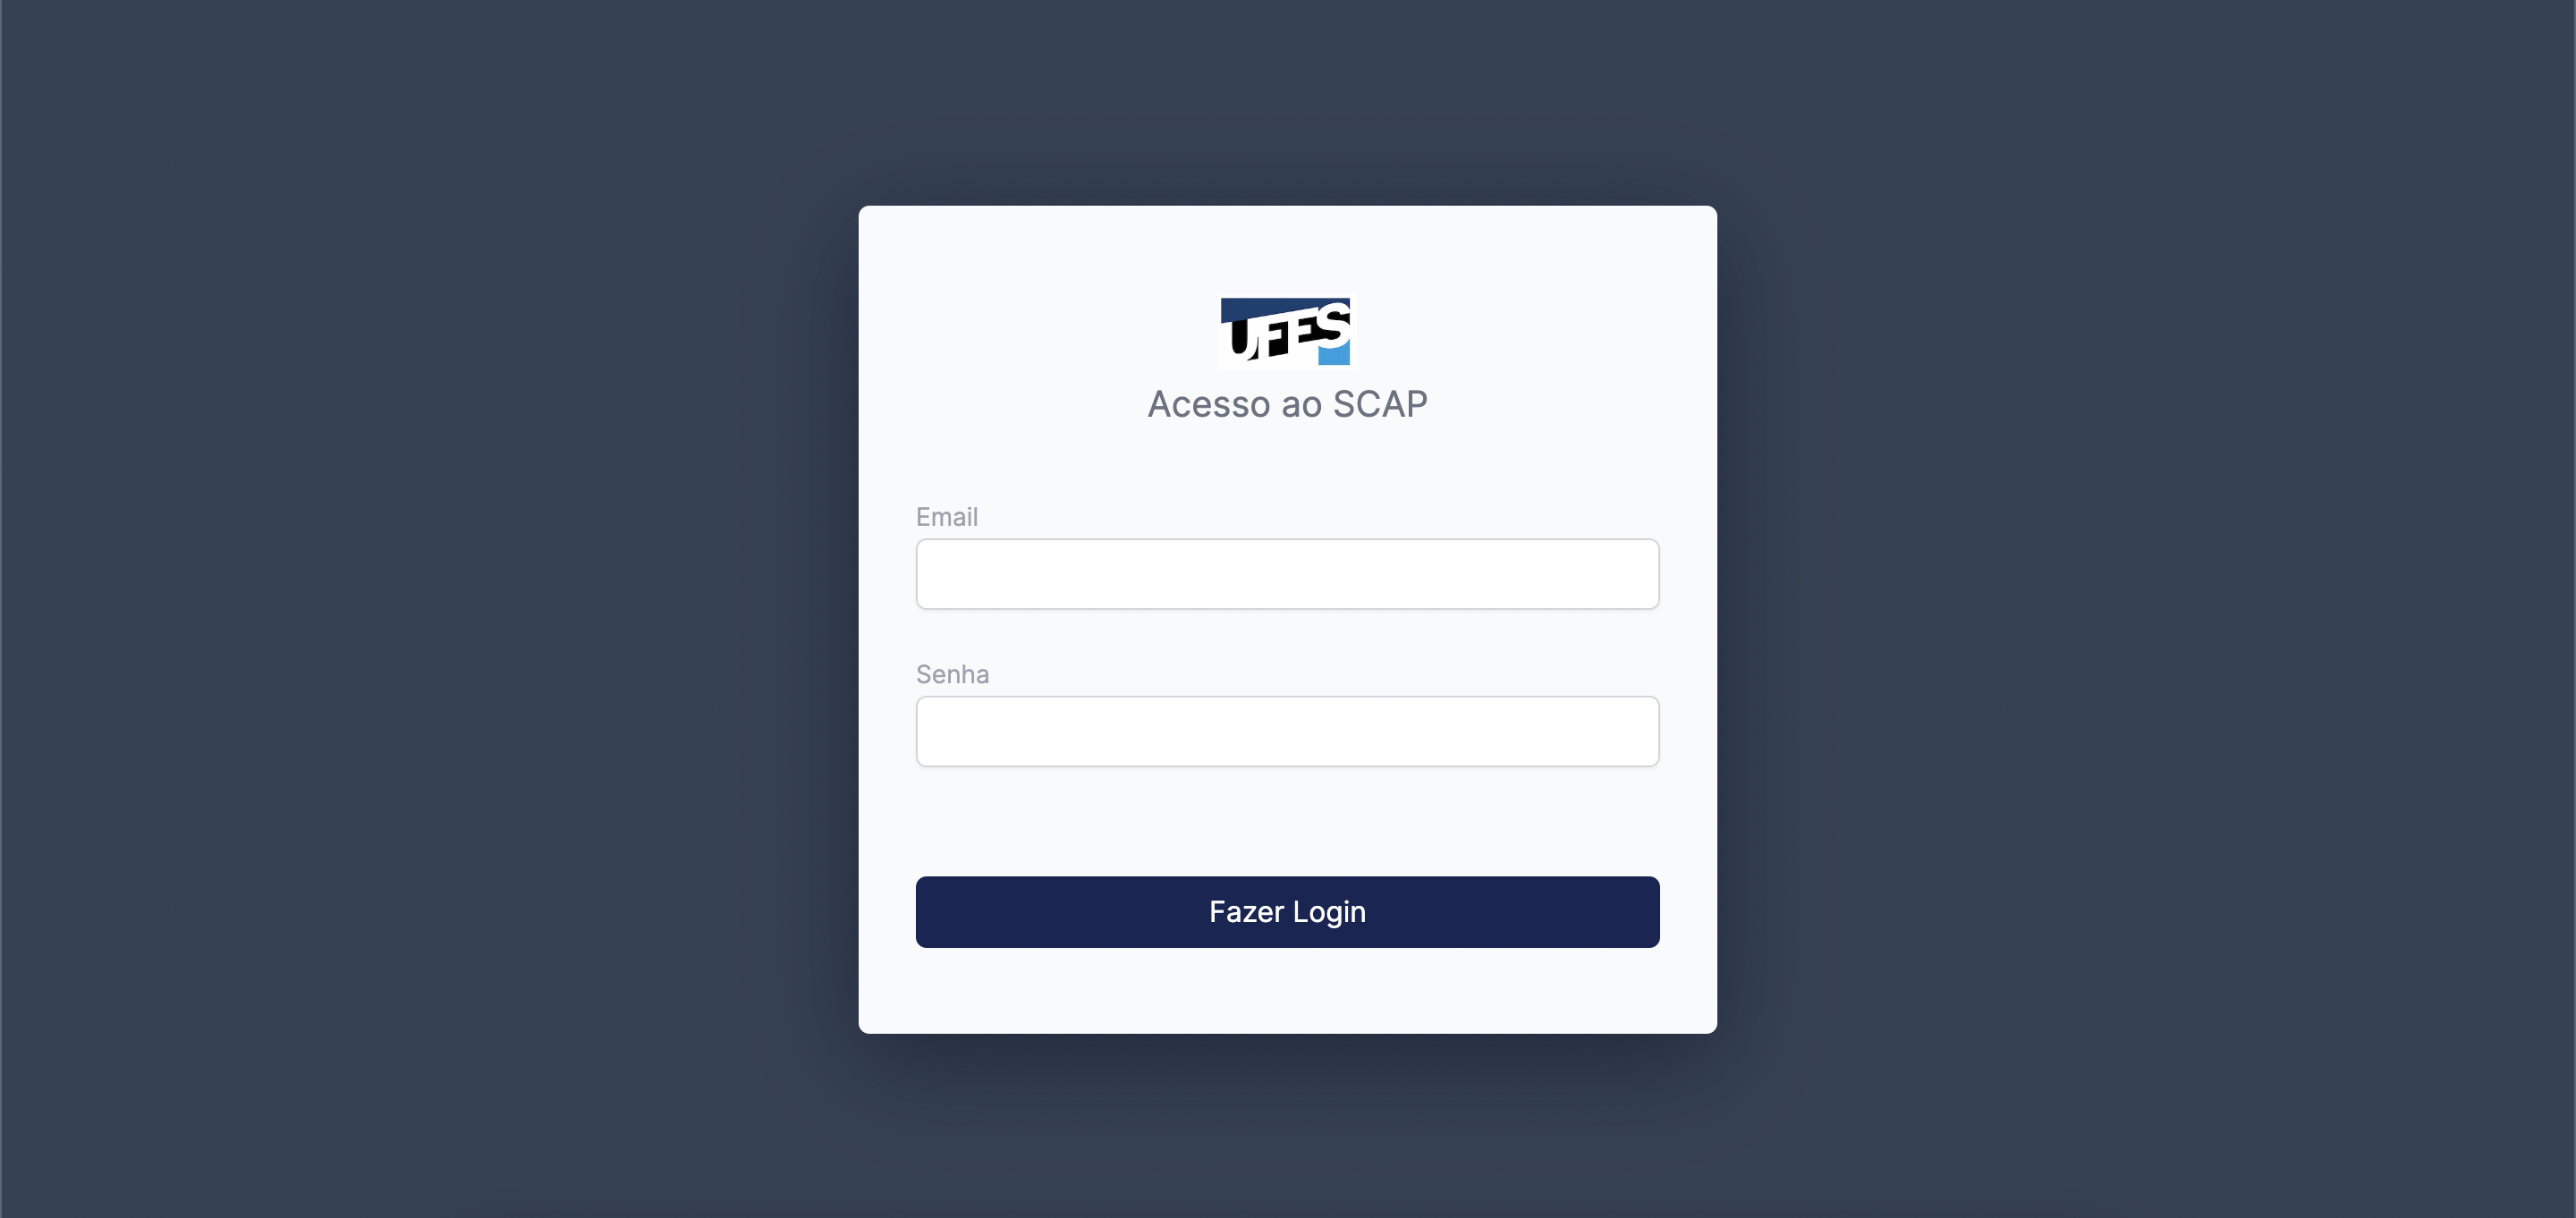
\includegraphics[width=\textwidth]{figuras/prints-app/fig-login.png}
    \caption{Tela de Login do SCAP.}
    \label{fig-login}
\end{figure}

Como mencionado anteriormente, existem dois tipos de usuários: secretário e professor. 
Os secretários são responsáveis por gerenciar os usuários e os estados dos afastamentos.
Já os professores podem solicitar afastamentos e visualizar o andamento das solicitações.
Dessa forma, as telas mudam de acordo com o tipo de usuário que está logado.


\subsection{Listagem de Afastamentos}
\label{subsec-projeto-afastamentos}

Ao completar o \textit{login}, o usuário é redirecionado para a página inicial do sistema, onde é possível
visualizar os afastamentos solicitados pelos professores. A Figura~\ref{fig-listagem-afastamentos} apresenta a tela de listagem de afastamentos
do SCAP. Nela é possível também buscar os afastamentos por diferentes critérios, como o nome do professor ou o estado do afastamento,
a Figura~\ref{fig-filtro-afastamentos} apresenta este filtro. Por fim, caso o usuário seja um professor,
o botão de solicitar afastamento estará disponível, ao clicá-lo o usuário é redirecionado para a página de cadastro de afastamento.

\begin{figure}[h!]
    \centering
    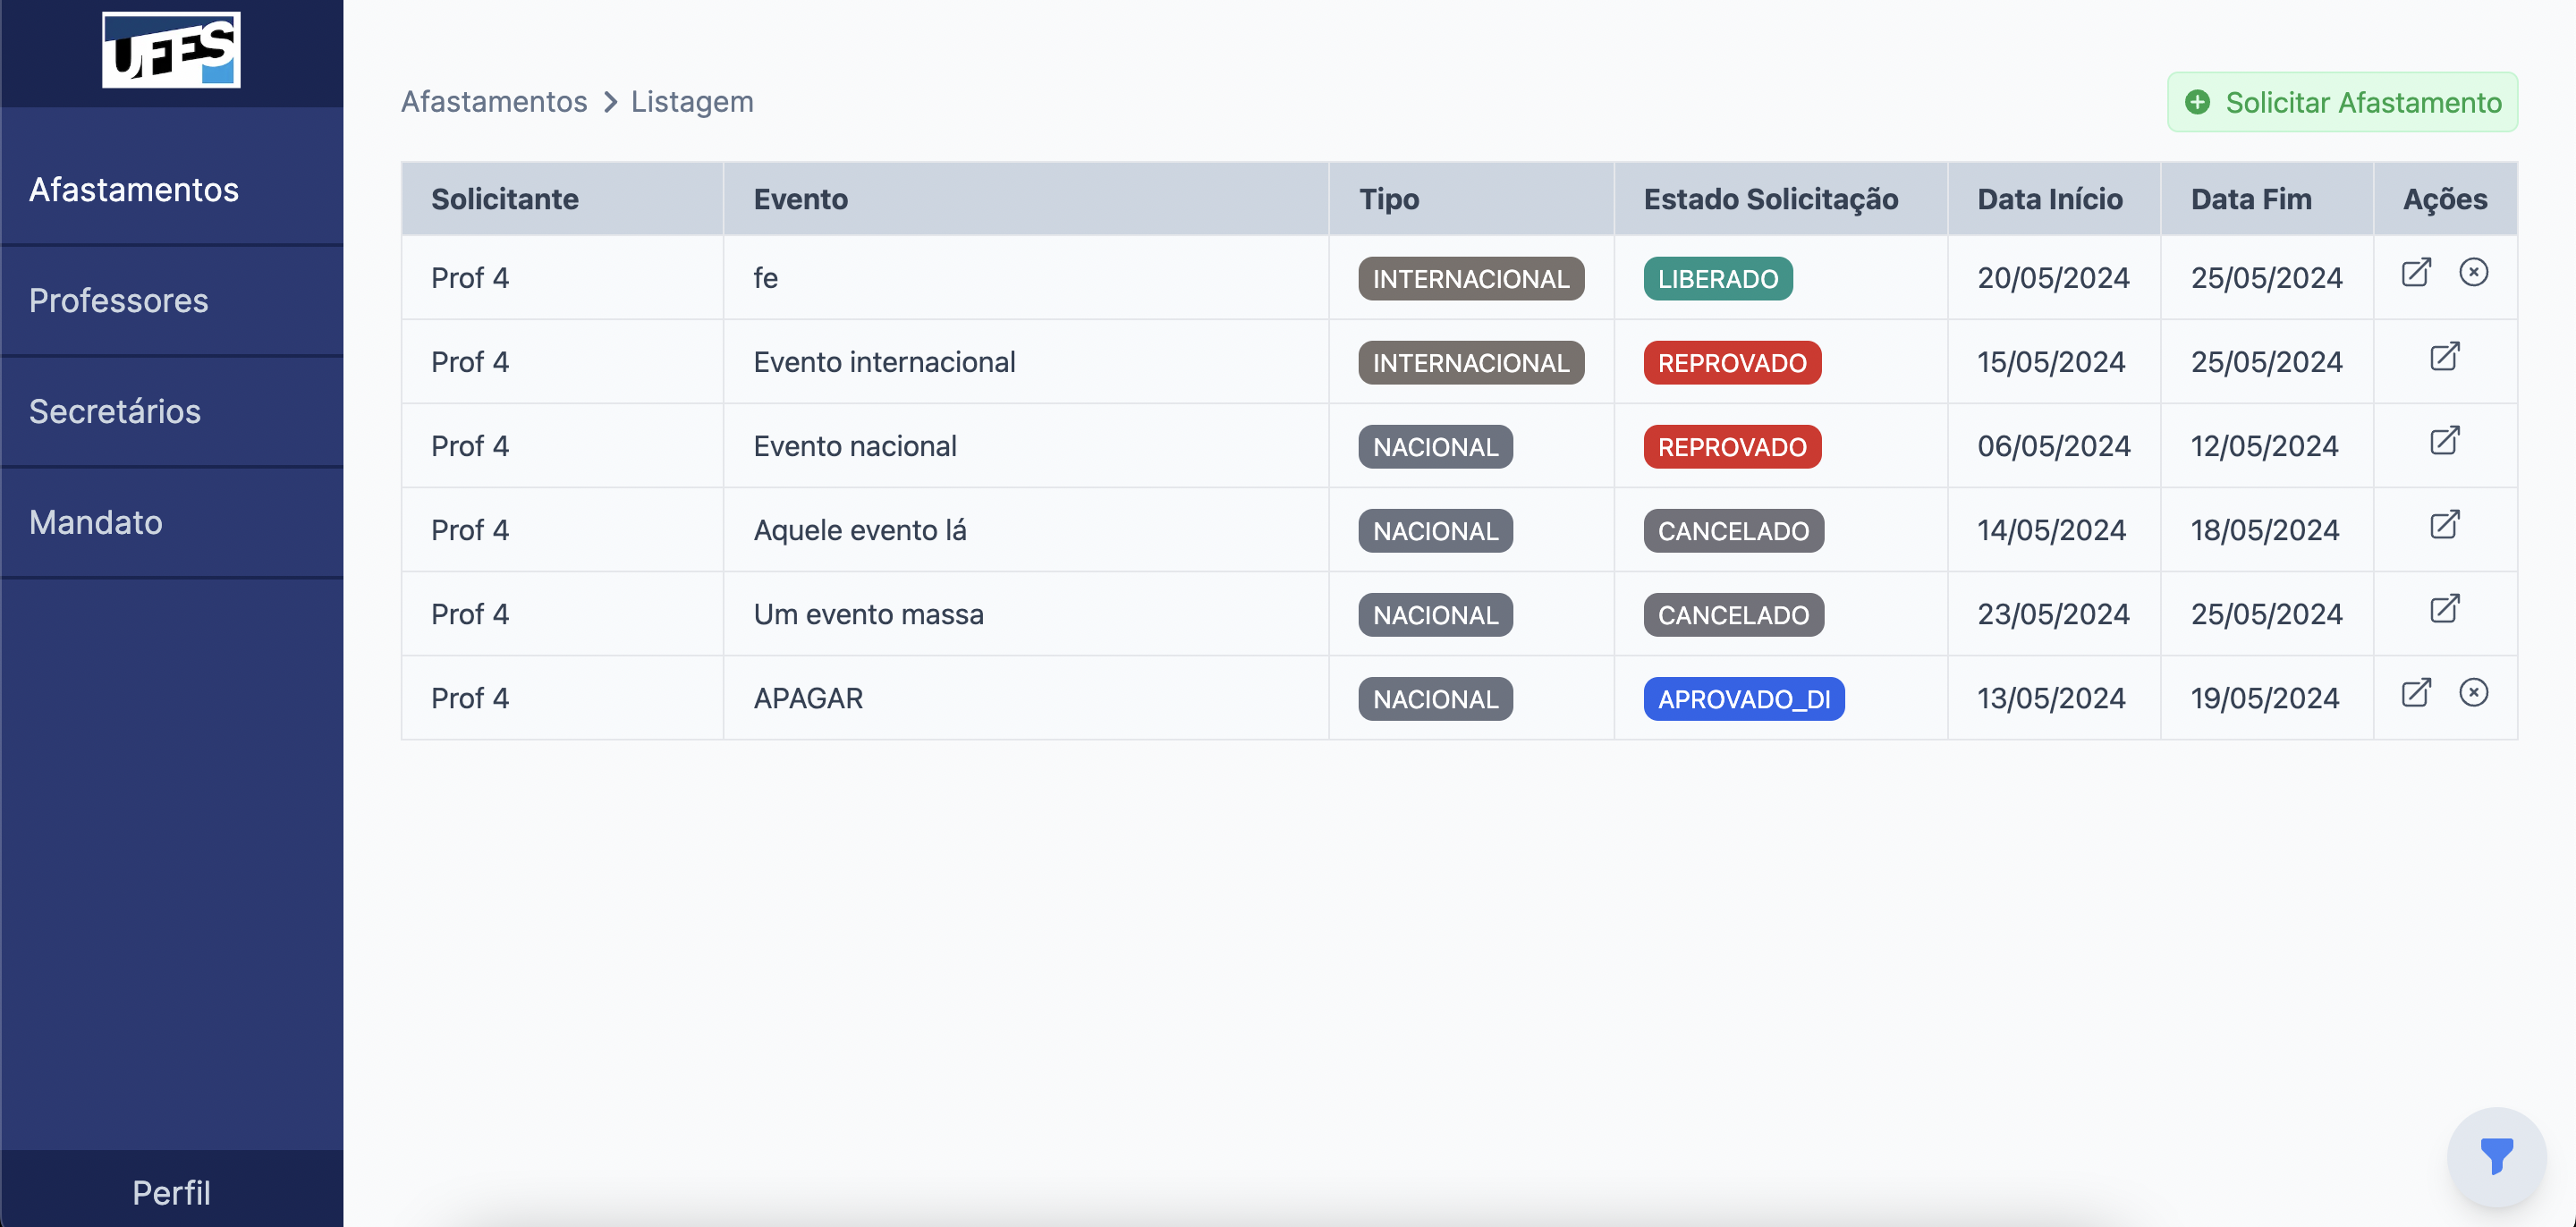
\includegraphics[width=\textwidth]{figuras/prints-app/fig-lista-afastamento.png}
    \caption{Listagem de Afastamentos do SCAP.}
    \label{fig-listagem-afastamentos}
\end{figure}

\begin{figure}[h!]
    \centering
    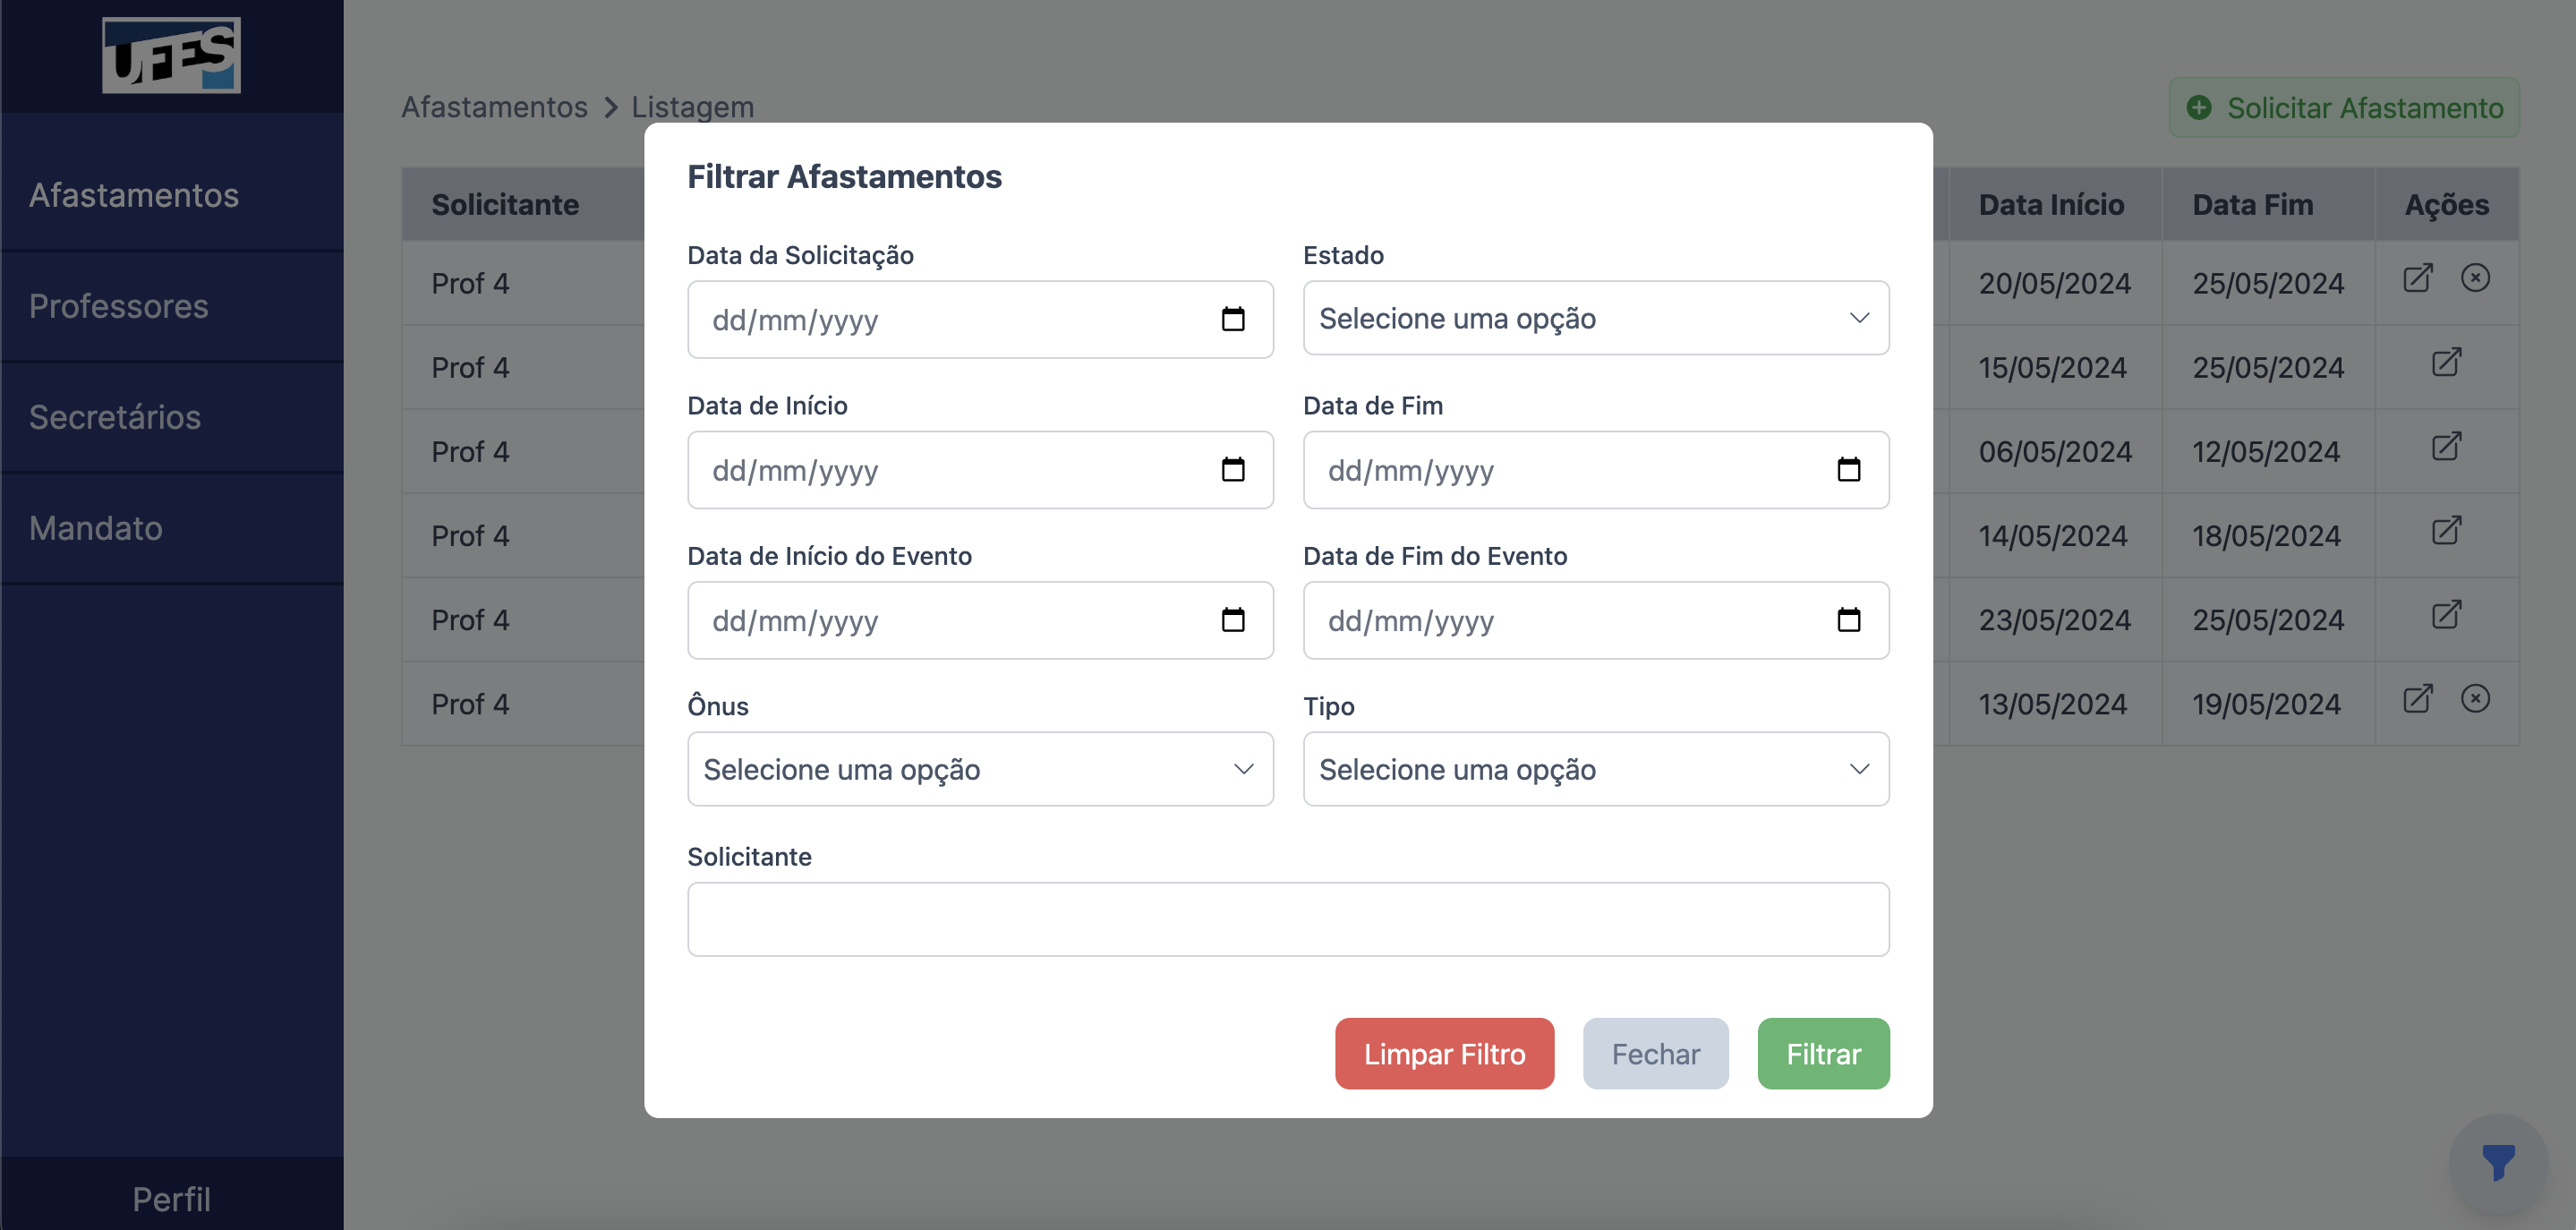
\includegraphics[width=\textwidth]{figuras/prints-app/fig-filtro-afastamento.png}
    \caption{Filtro de Busca de Afastamentos.}
    \label{fig-filtro-afastamentos}
\end{figure}

\subsection{Cadastro de Afastamento}
\label{subsec-projeto-cadastro-afastamento}

A Figura~\ref{fig-cadastro-afastamento} apresenta a tela de cadastro de afastamento do SCAP. Esta rota
é acessível apenas para professores, que podem solicitar um afastamento preenchendo o formulário,
campos marcados com asterisco são obrigatórios. 

\begin{figure}[h!]
    \centering
    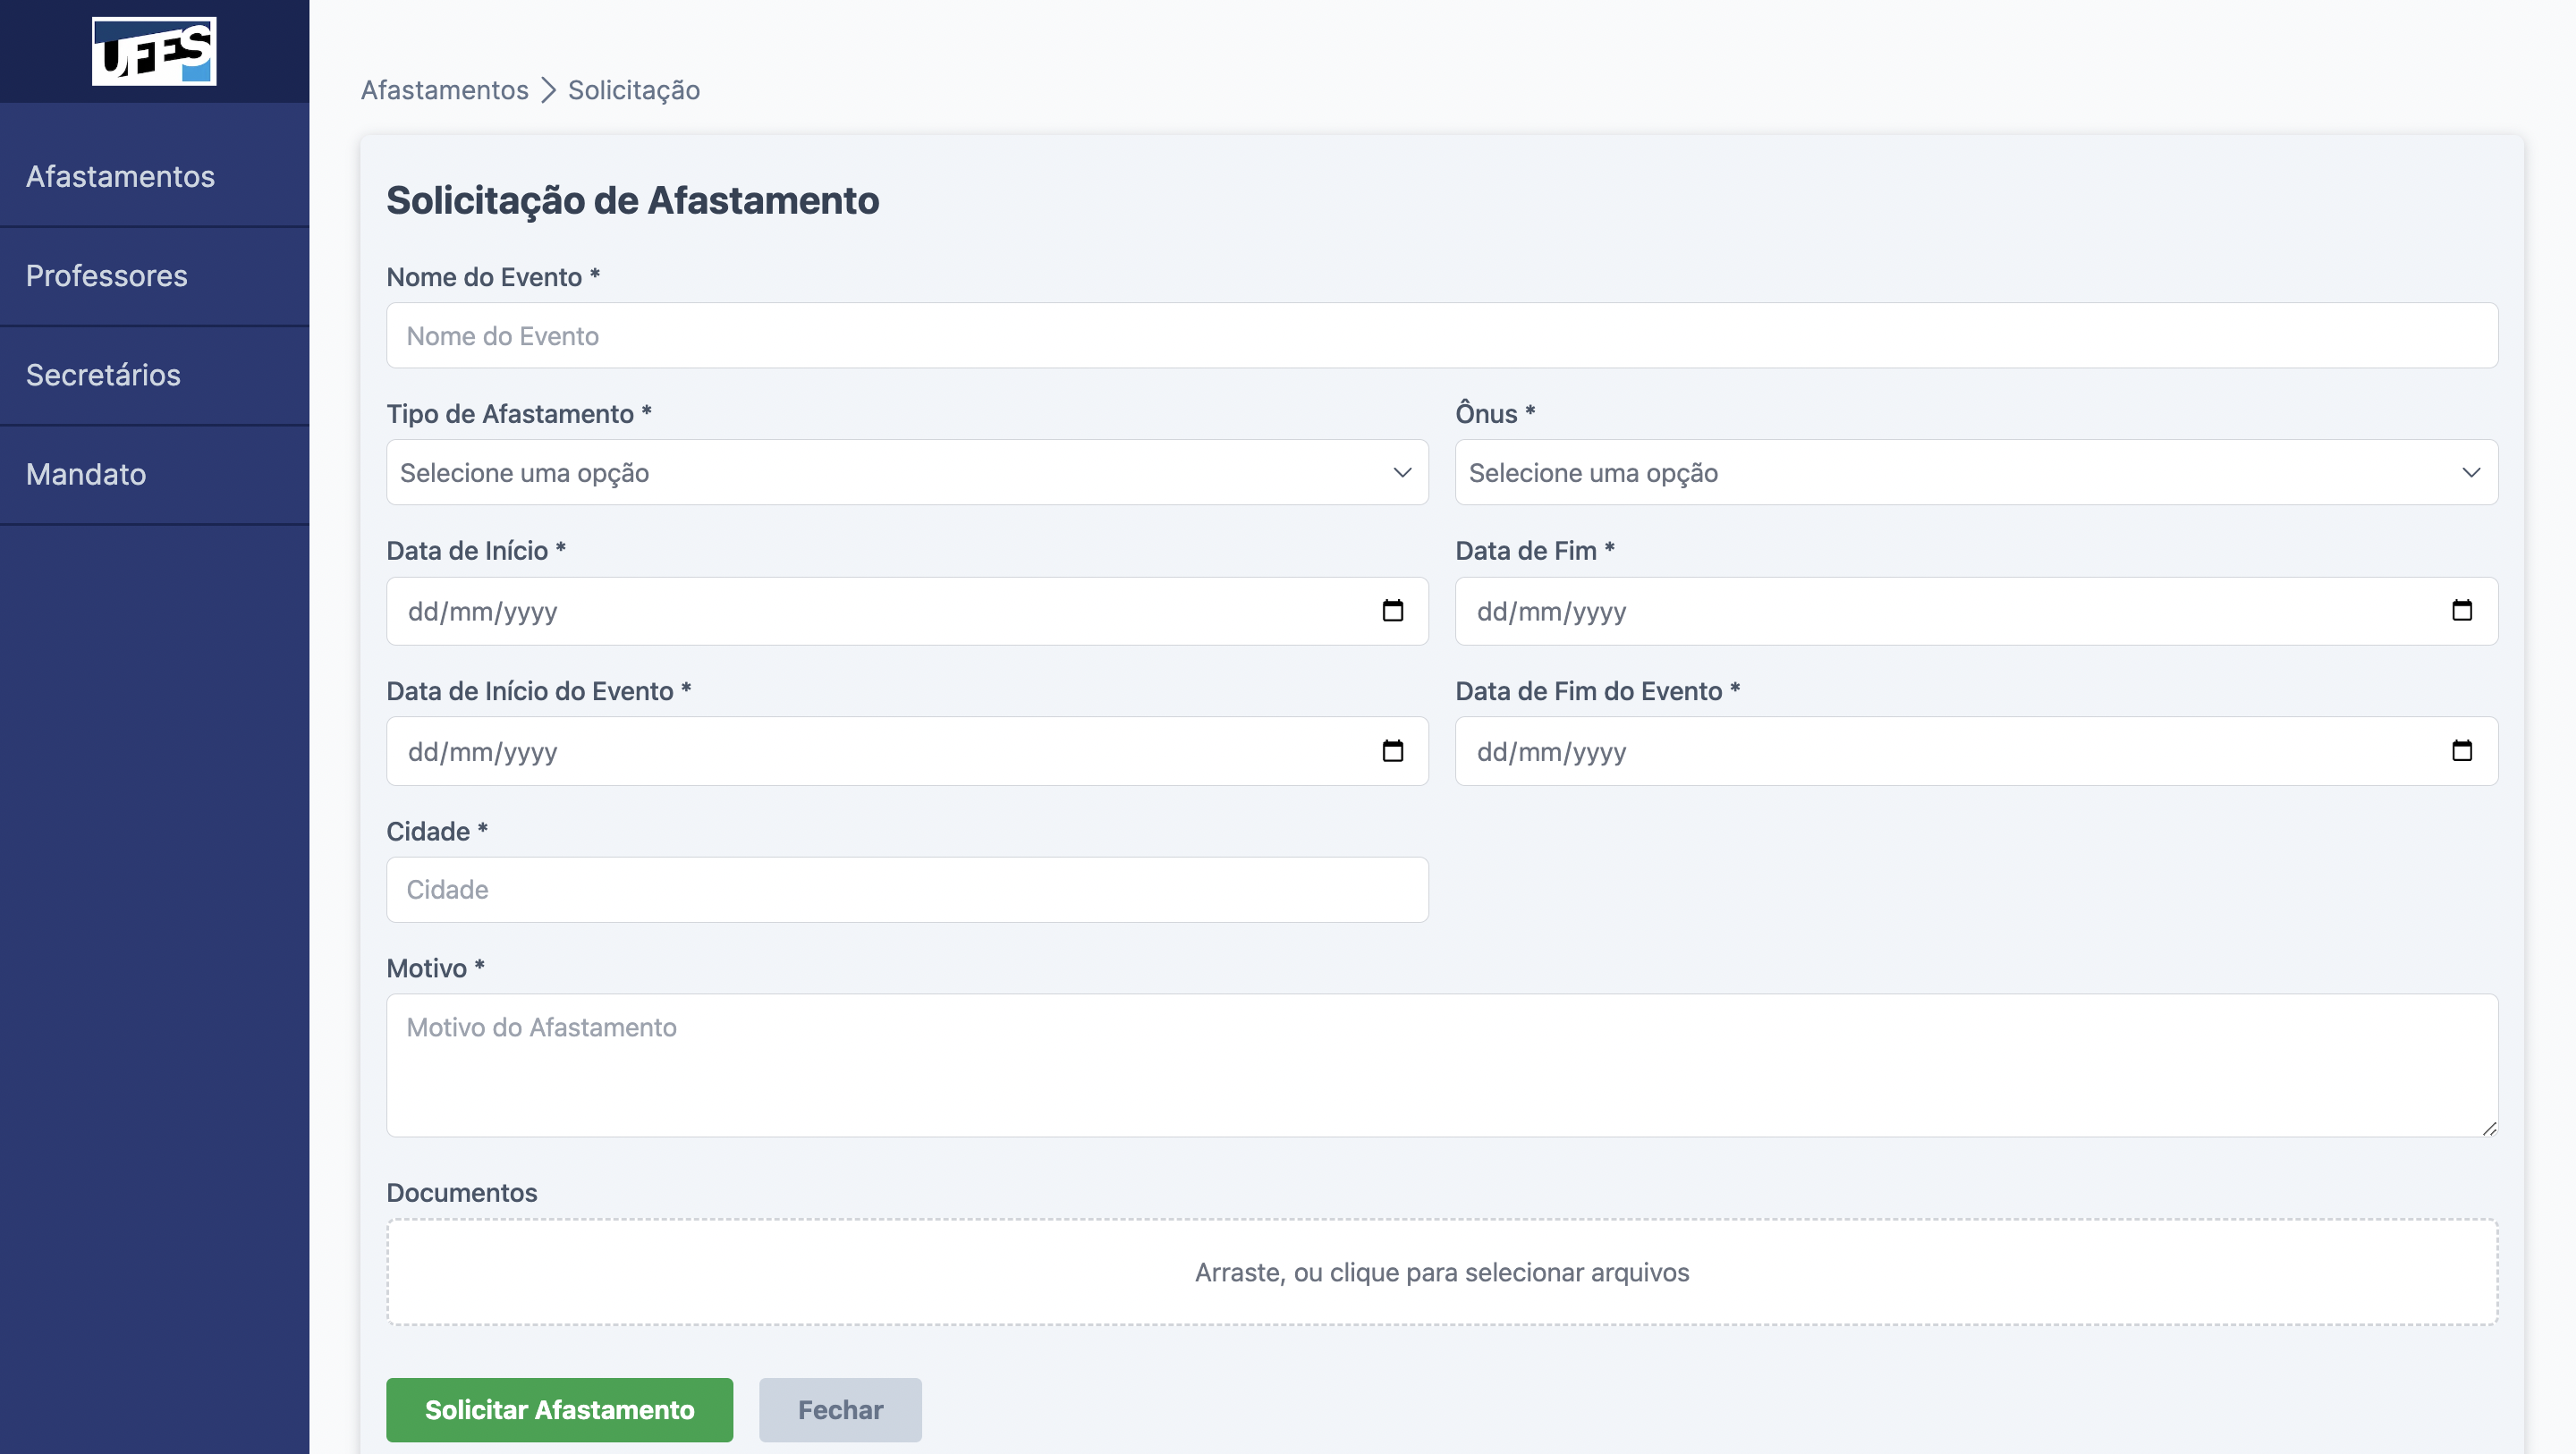
\includegraphics[width=\textwidth]{figuras/prints-app/fig-solicitar-afastamento.png}
    \caption{Cadastro de Afastamento do SCAP.}
    \label{fig-cadastro-afastamento}
\end{figure}

A edição de um afastamento é feita de forma similar ao cadastro, porém os campos já estarão preenchidos com os valores
do afastamento a ser editado. O mesmo componente é utilizado para ambas as ações, estando a diferença na rota acessada.
Na edição, apenas o professor solicitante pode editar as informações do afastamento, exceto os campos:
\textit{estado} e \textit{relator}, que são de responsabilidade do secretário e professor chefe, respectivamente.

\begin{figure}
    \centering
    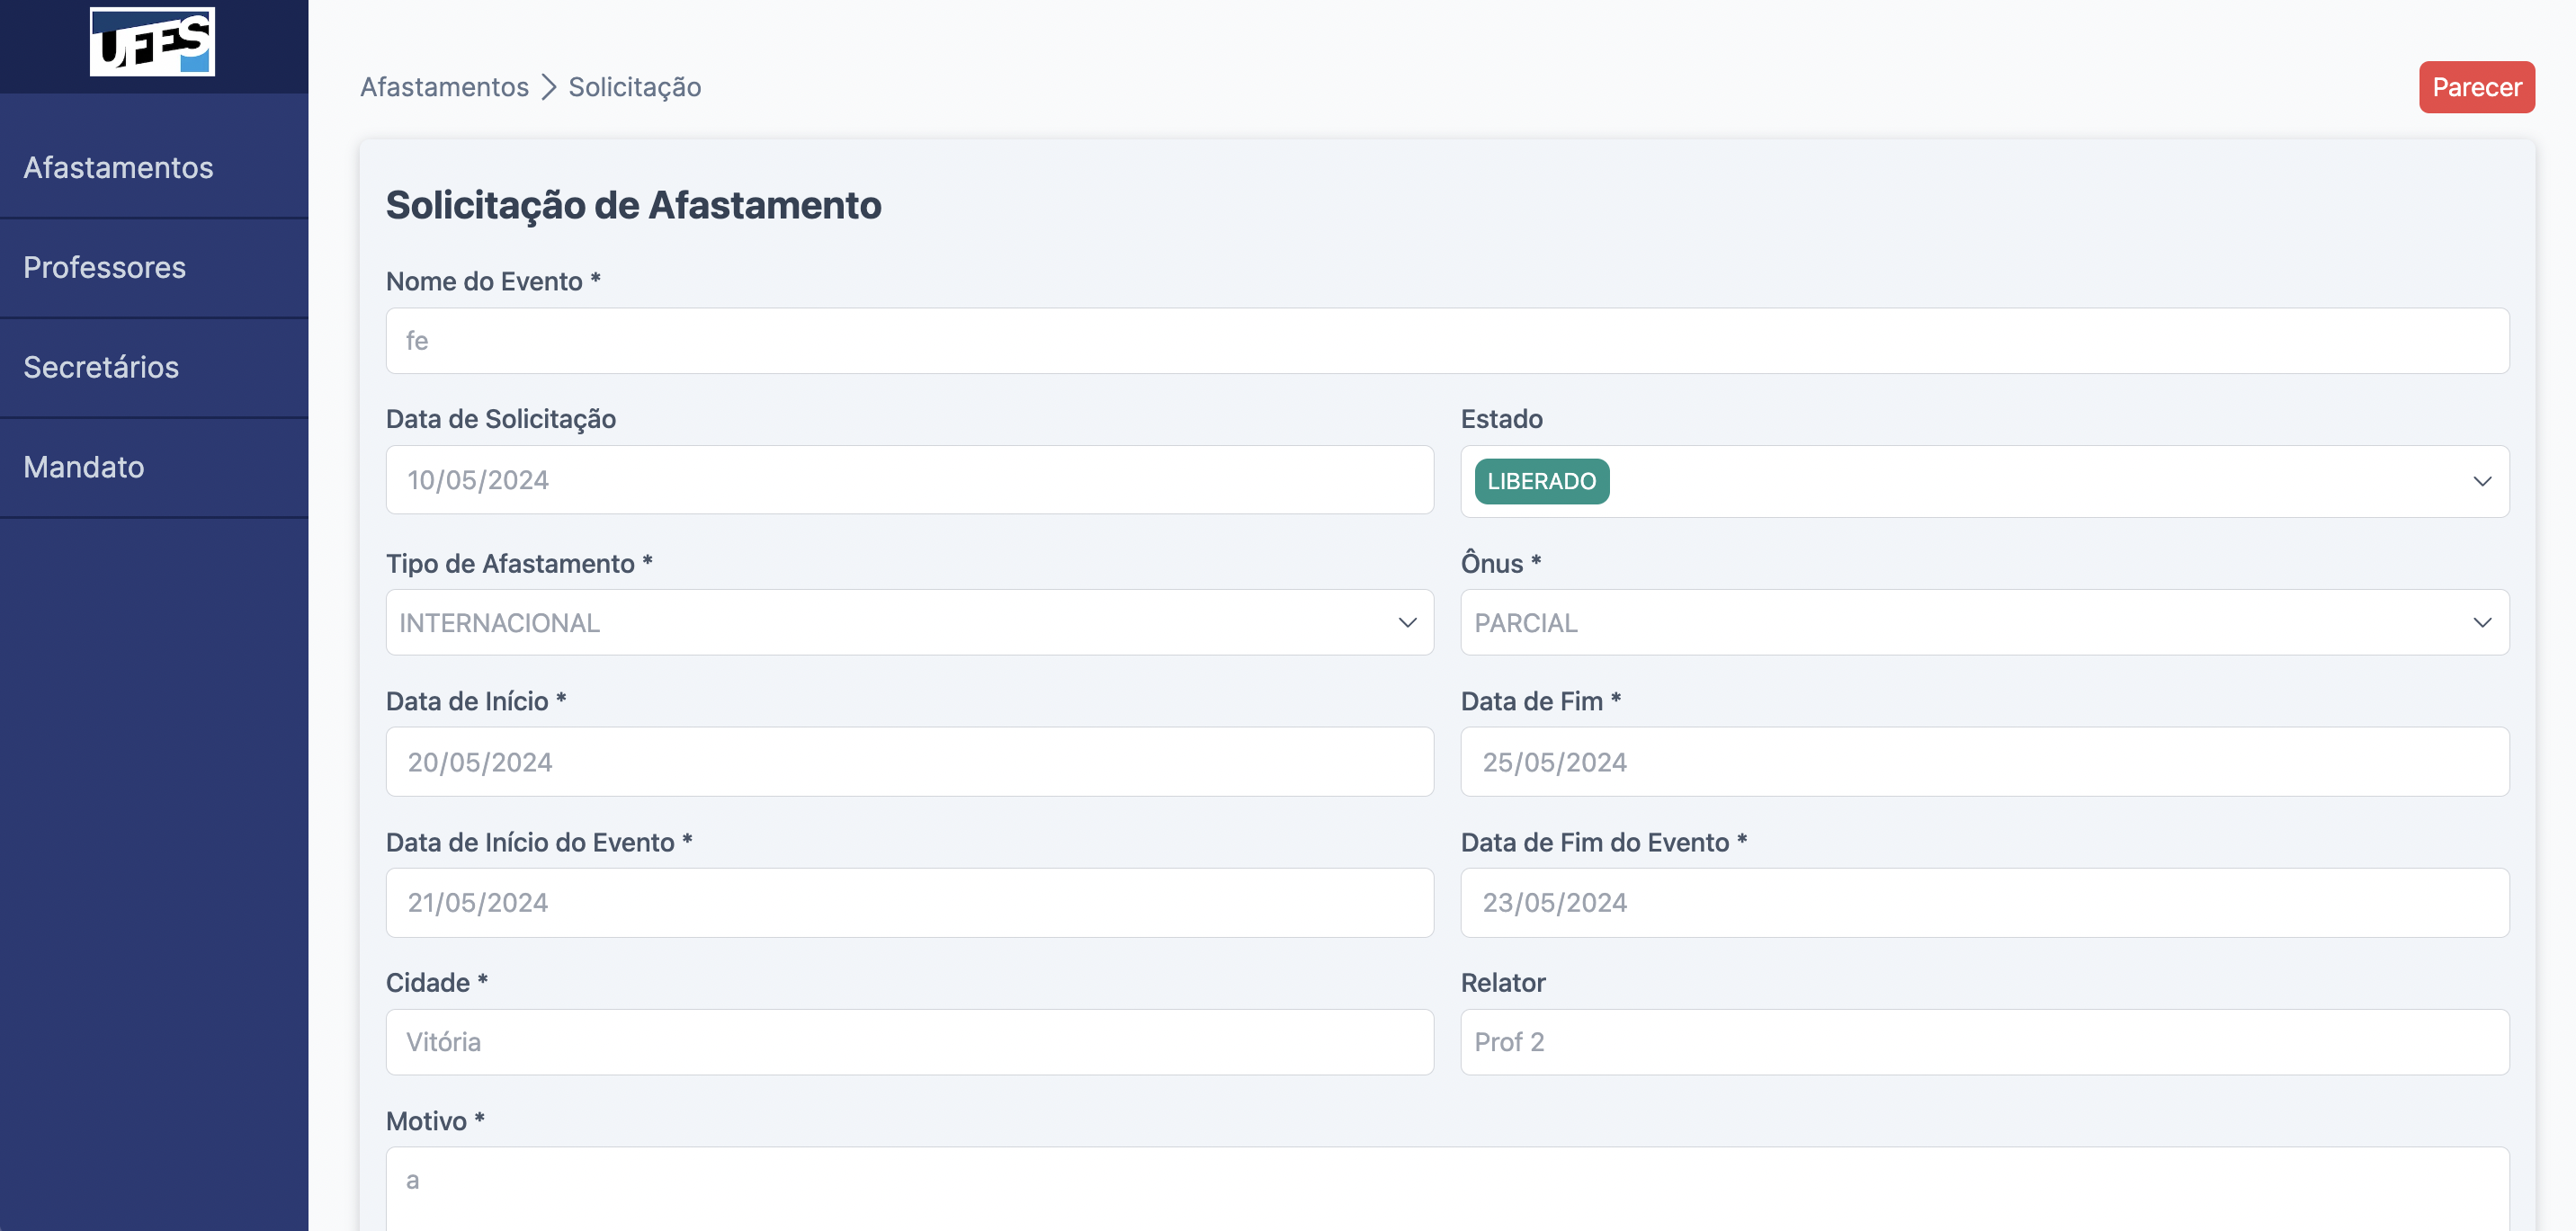
\includegraphics[width=\textwidth]{figuras/prints-app/fig-editar-afastamento.png}
    \caption{Edição de Afastamento do SCAP.}
    \label{fig-editar-afastamento}
\end{figure}

Caso seja um professor sem parentesco com o solicitante do afastamento, o botão de \textbf{Parecer} estará disponível,
abrindo um modal com o formulário para preenchimento do parecer. A Figura~\ref{fig-parecer} apresenta este modal.
Por serem funcionalidades semelhantes, o modal de parecer é utilizado também para pareceres externos (CT e PRPPG) e manifestações
de professores contra o afastamento nacional.

\begin{figure}
    \centering
    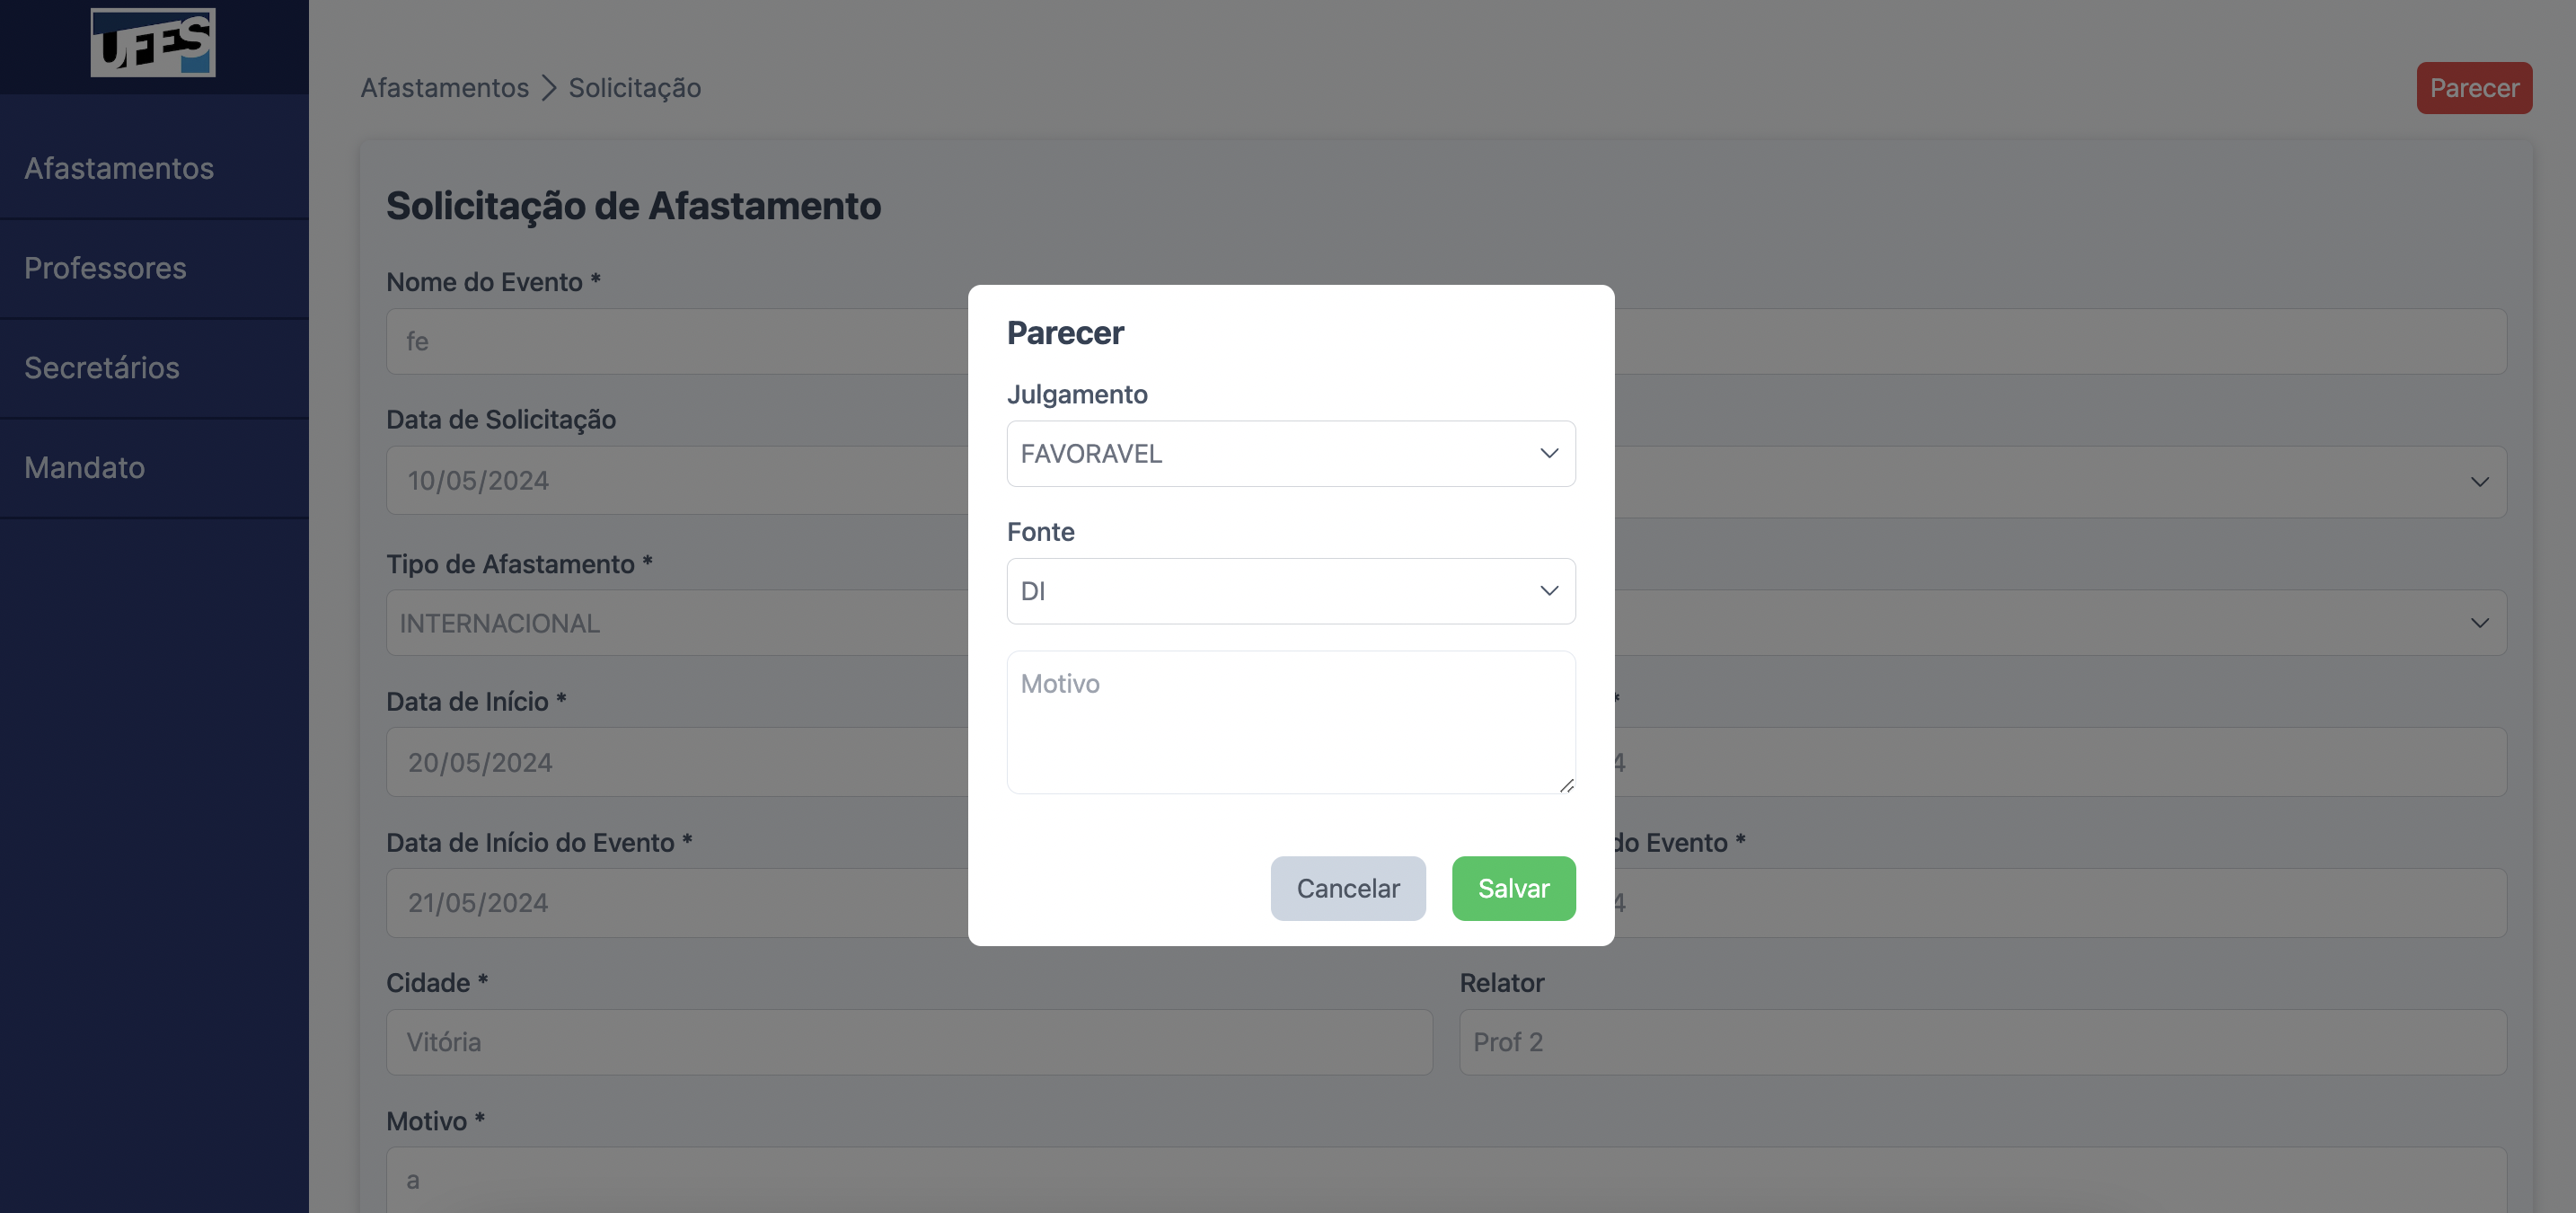
\includegraphics[width=\textwidth]{figuras/prints-app/fig-parecer.png}
    \caption{Modal de Parecer do SCAP.}
    \label{fig-parecer}
\end{figure}

Por fim, o formulário de afastamento possui também um campo para \textit{upload} de arquivos, onde o professor solicitante
pode anexar o relatório de viagem e o secretário pode anexar atas ou documentos enviados pelo CT e PRPPG.

\subsection{Cadastro de Usuários}
\label{subsec-projeto-cadastro-usuarios}

Através do \textbf{NavBar} é possível navegar pela aplicação, clicando em \textbf{Professores} o usuário é redirecionado
para a página de listagem de professores, onde é possível visualizar os professores cadastrados, assim como seus \textit{e-mails}
e telefones. A Figura~\ref{fig-listagem-professores} apresenta a tela de listagem de professores do SCAP.

\begin{figure}[h!]
    \centering
    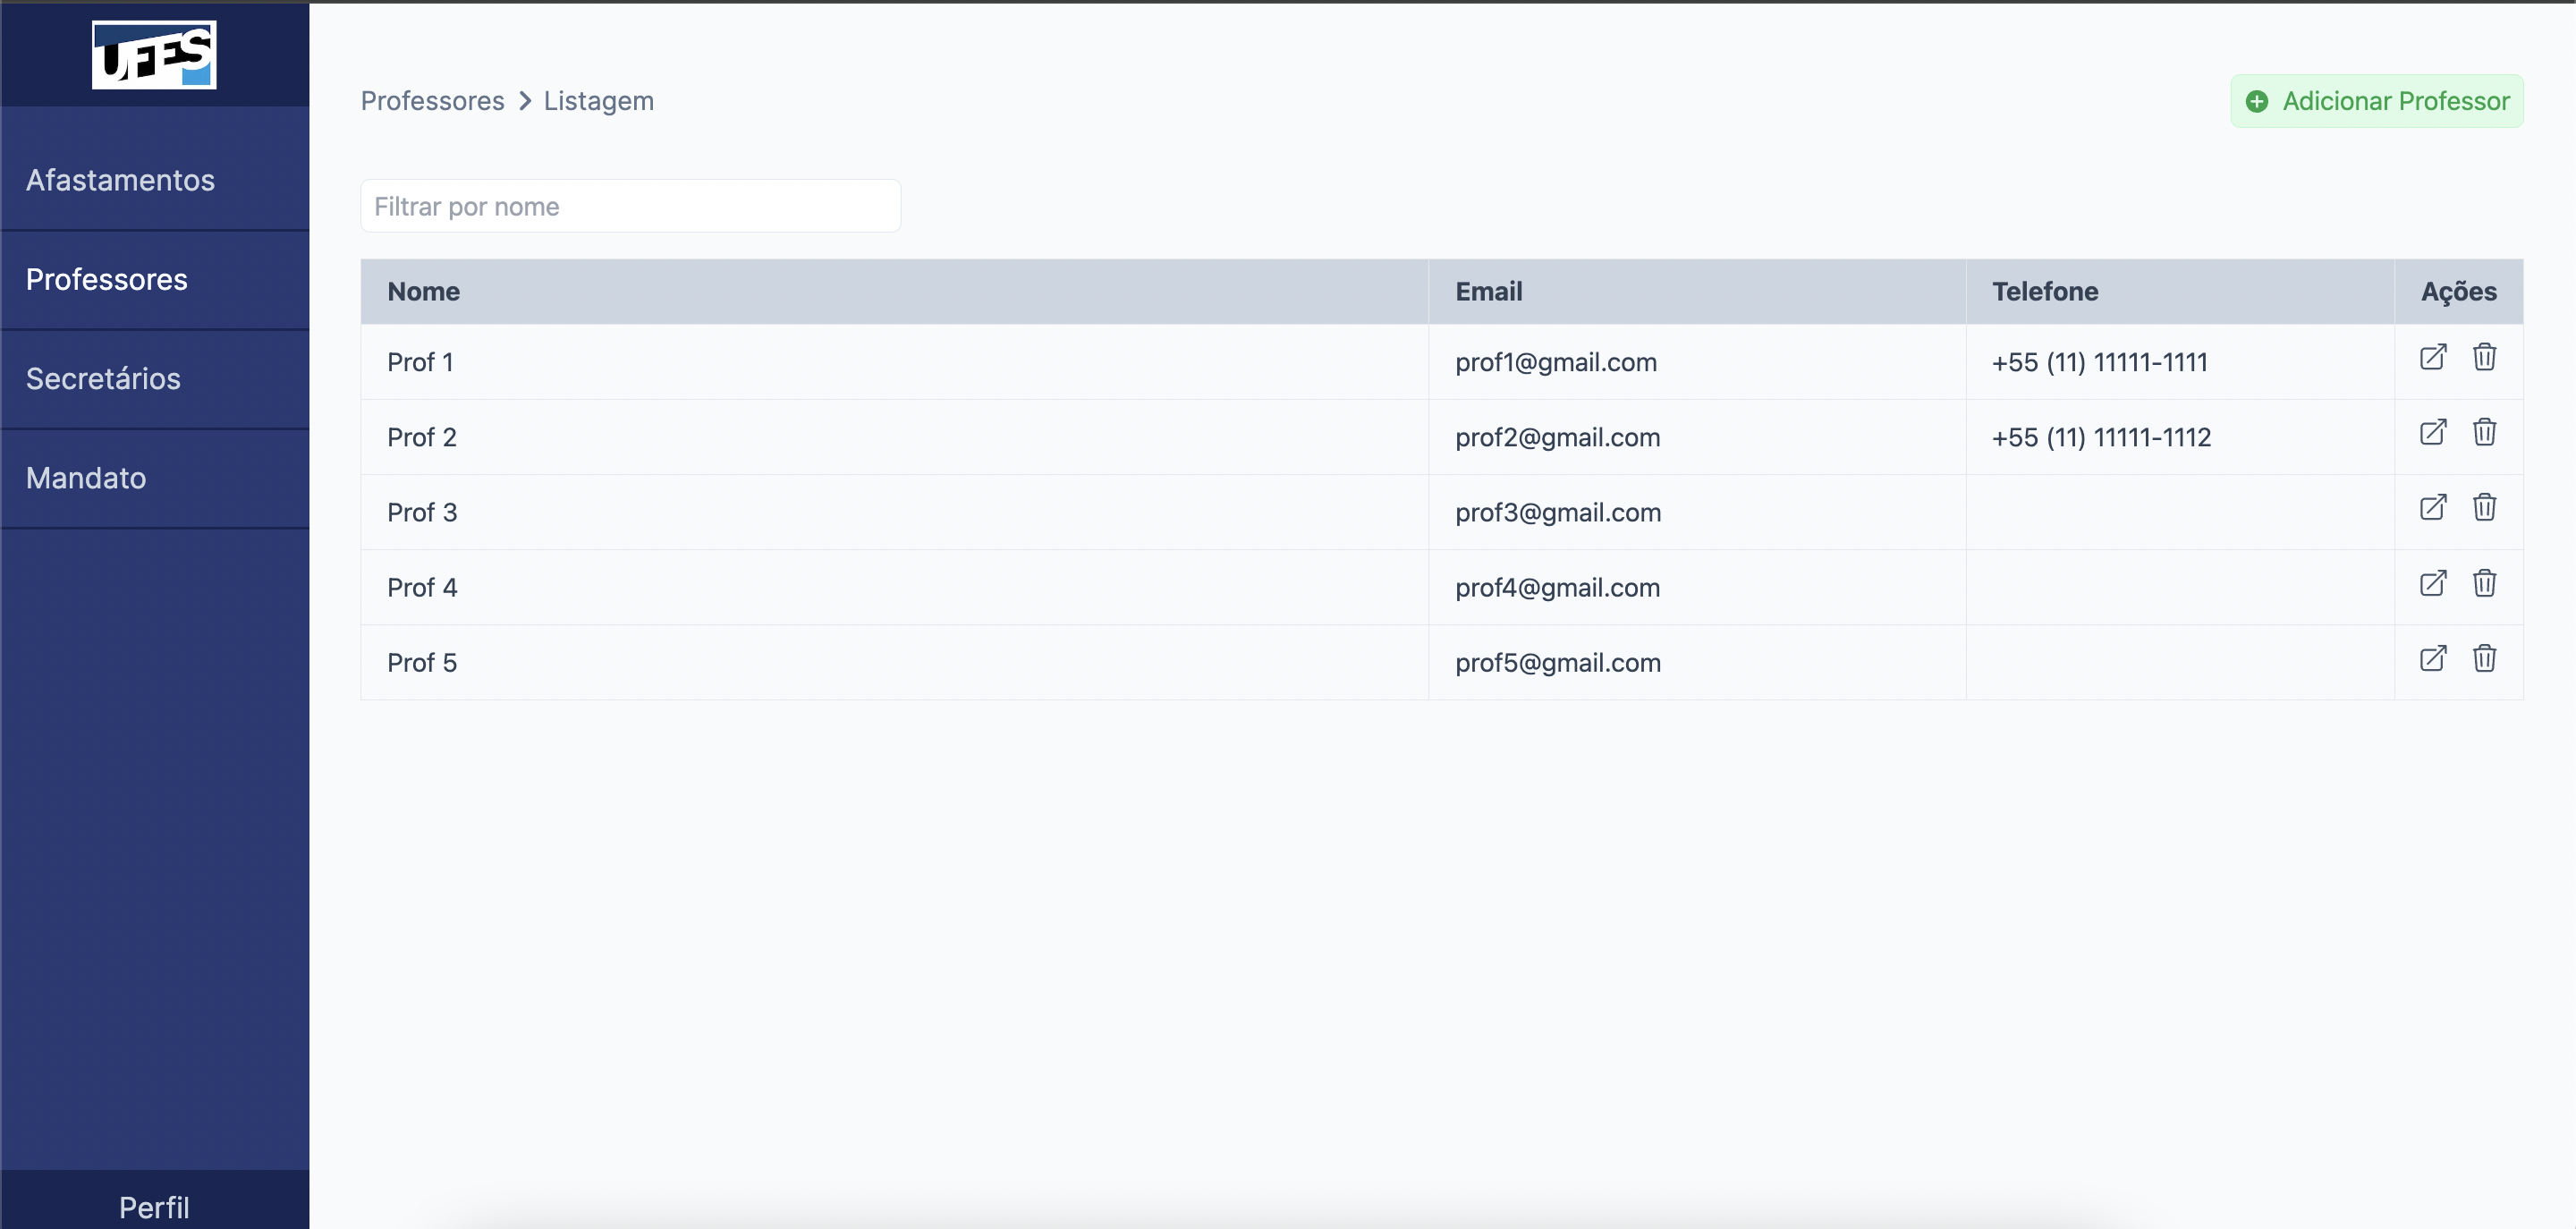
\includegraphics[width=\textwidth]{figuras/prints-app/fig-lista-professor.png}
    \caption{Listagem de Professores do SCAP.}
    \label{fig-listagem-professores}
\end{figure}

A Figura~\ref{fig-listagem-secretarios} apresenta a tela de listagem de secretários, que pode ser acessada
da mesma forma, pelo \textbf{NavBar} clicando em \textbf{Secretários}.

\begin{figure}[h!]
    \centering
    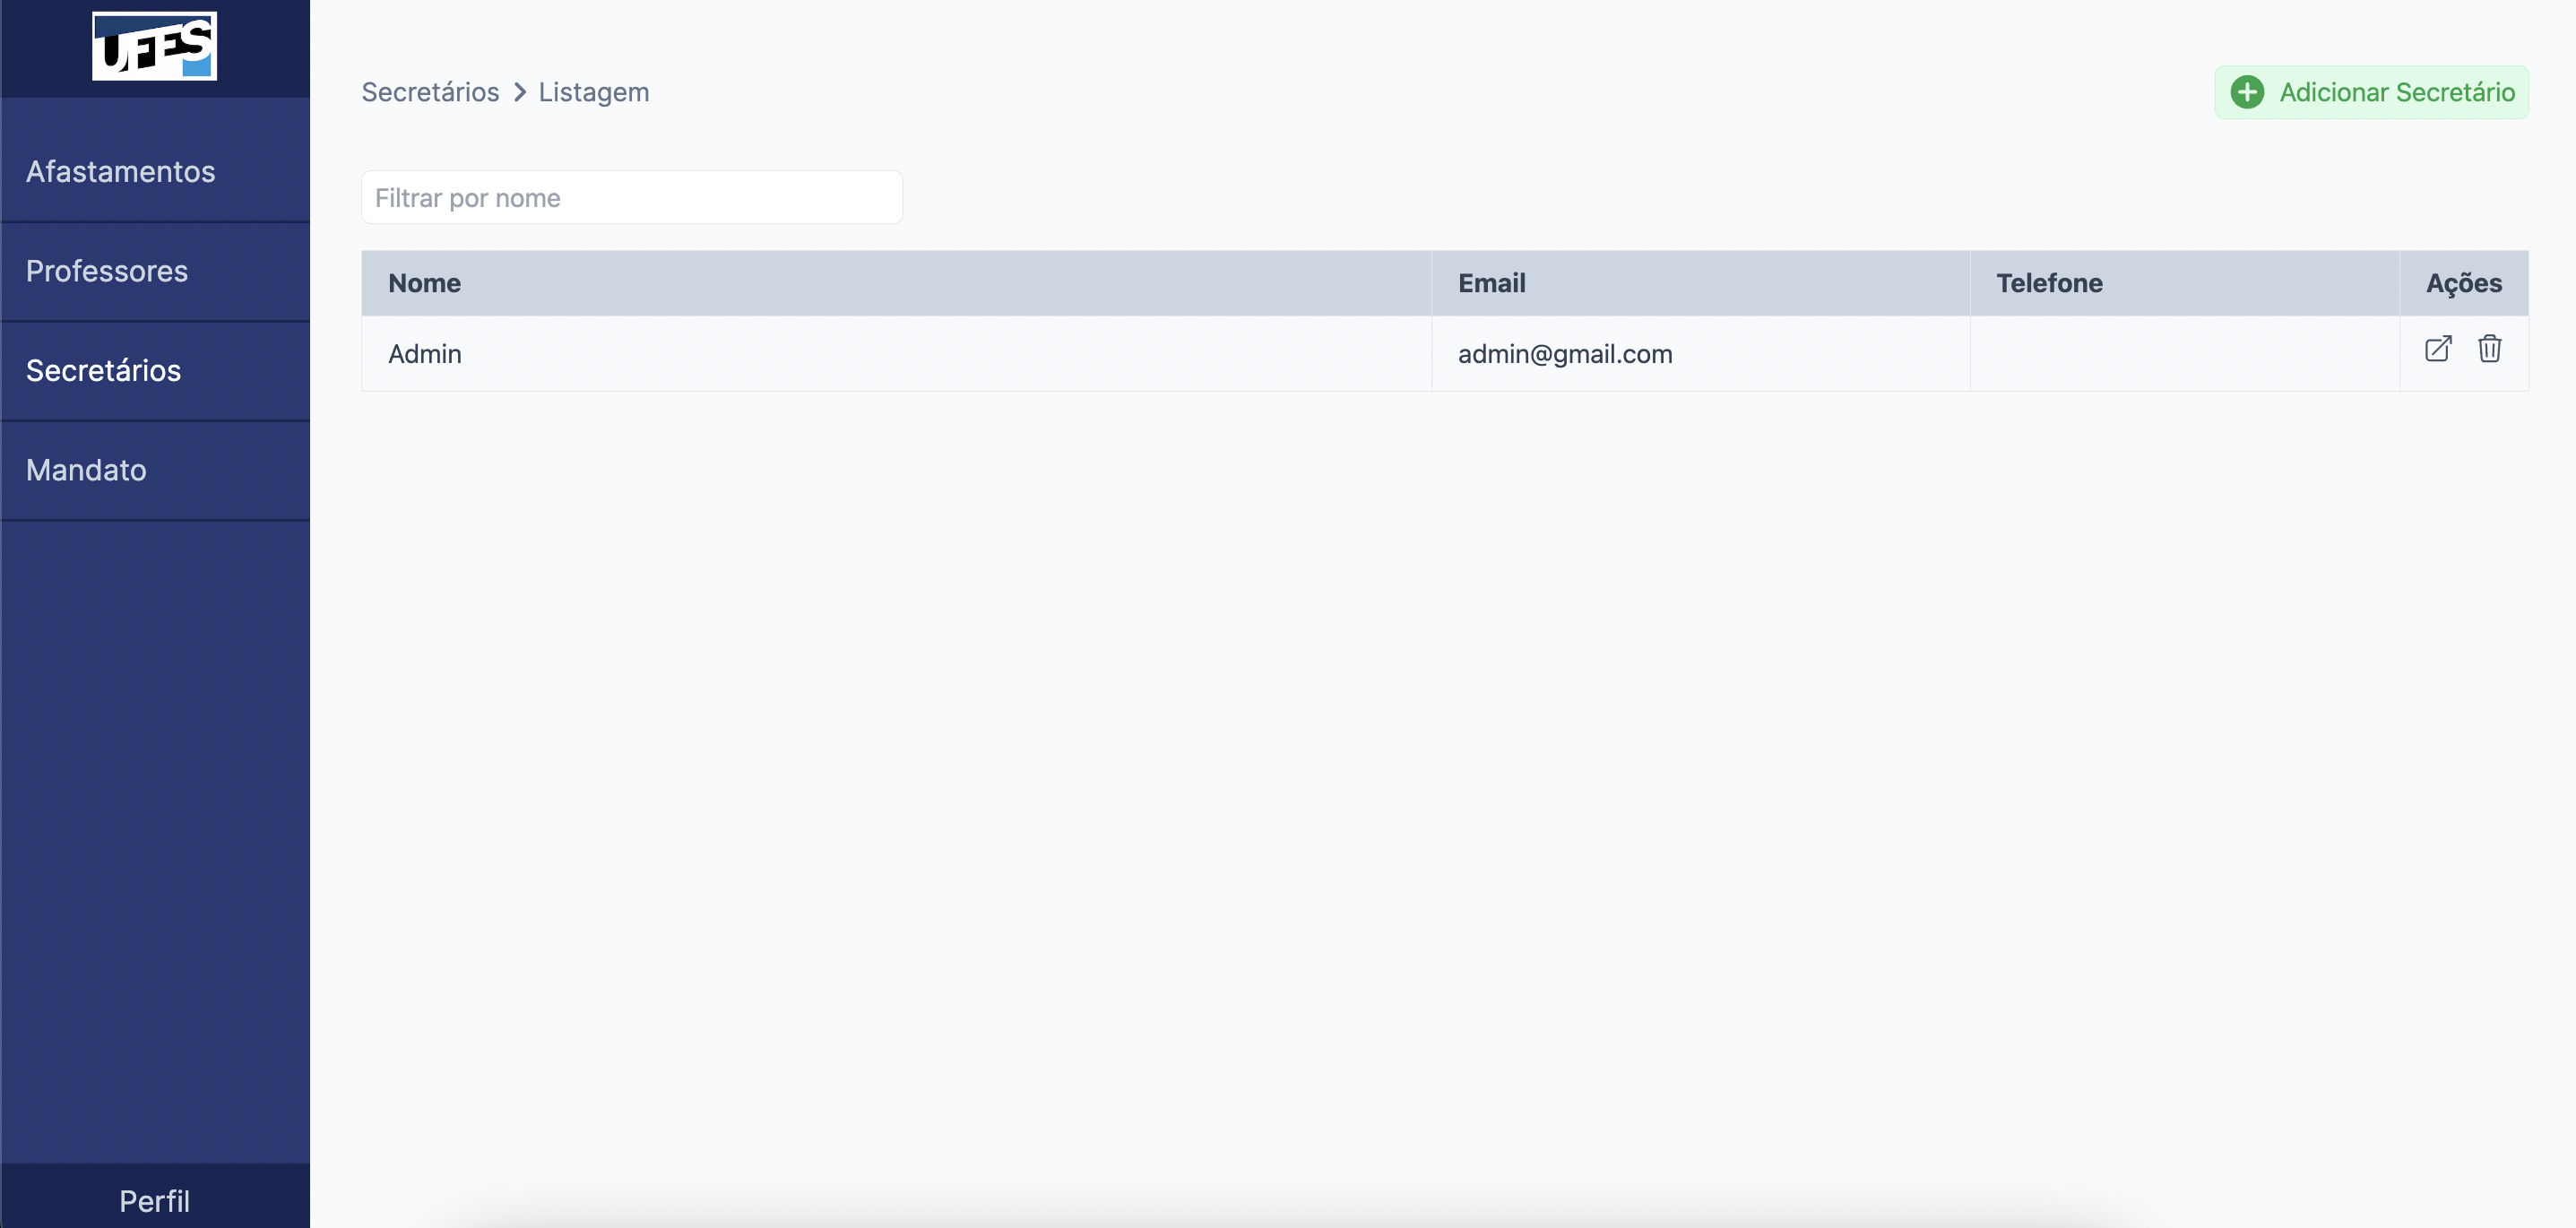
\includegraphics[width=\textwidth]{figuras/prints-app/fig-lista-secretario.png}
    \caption{Listagem de Secretários do SCAP.}
    \label{fig-listagem-secretarios}
\end{figure}

Apenas o secretário pode deletar, visualizar e adicionar professores. A Figura~\ref{fig-cadastro-professor} apresenta
a tela de cadastro de usuários, por onde o secretário pode adicionar um novo usuário preenchendo o formulário,
seja ele um professor ou secretário. Campos marcados com asterisco são obrigatórios.

\begin{figure}[h!]
    \centering
    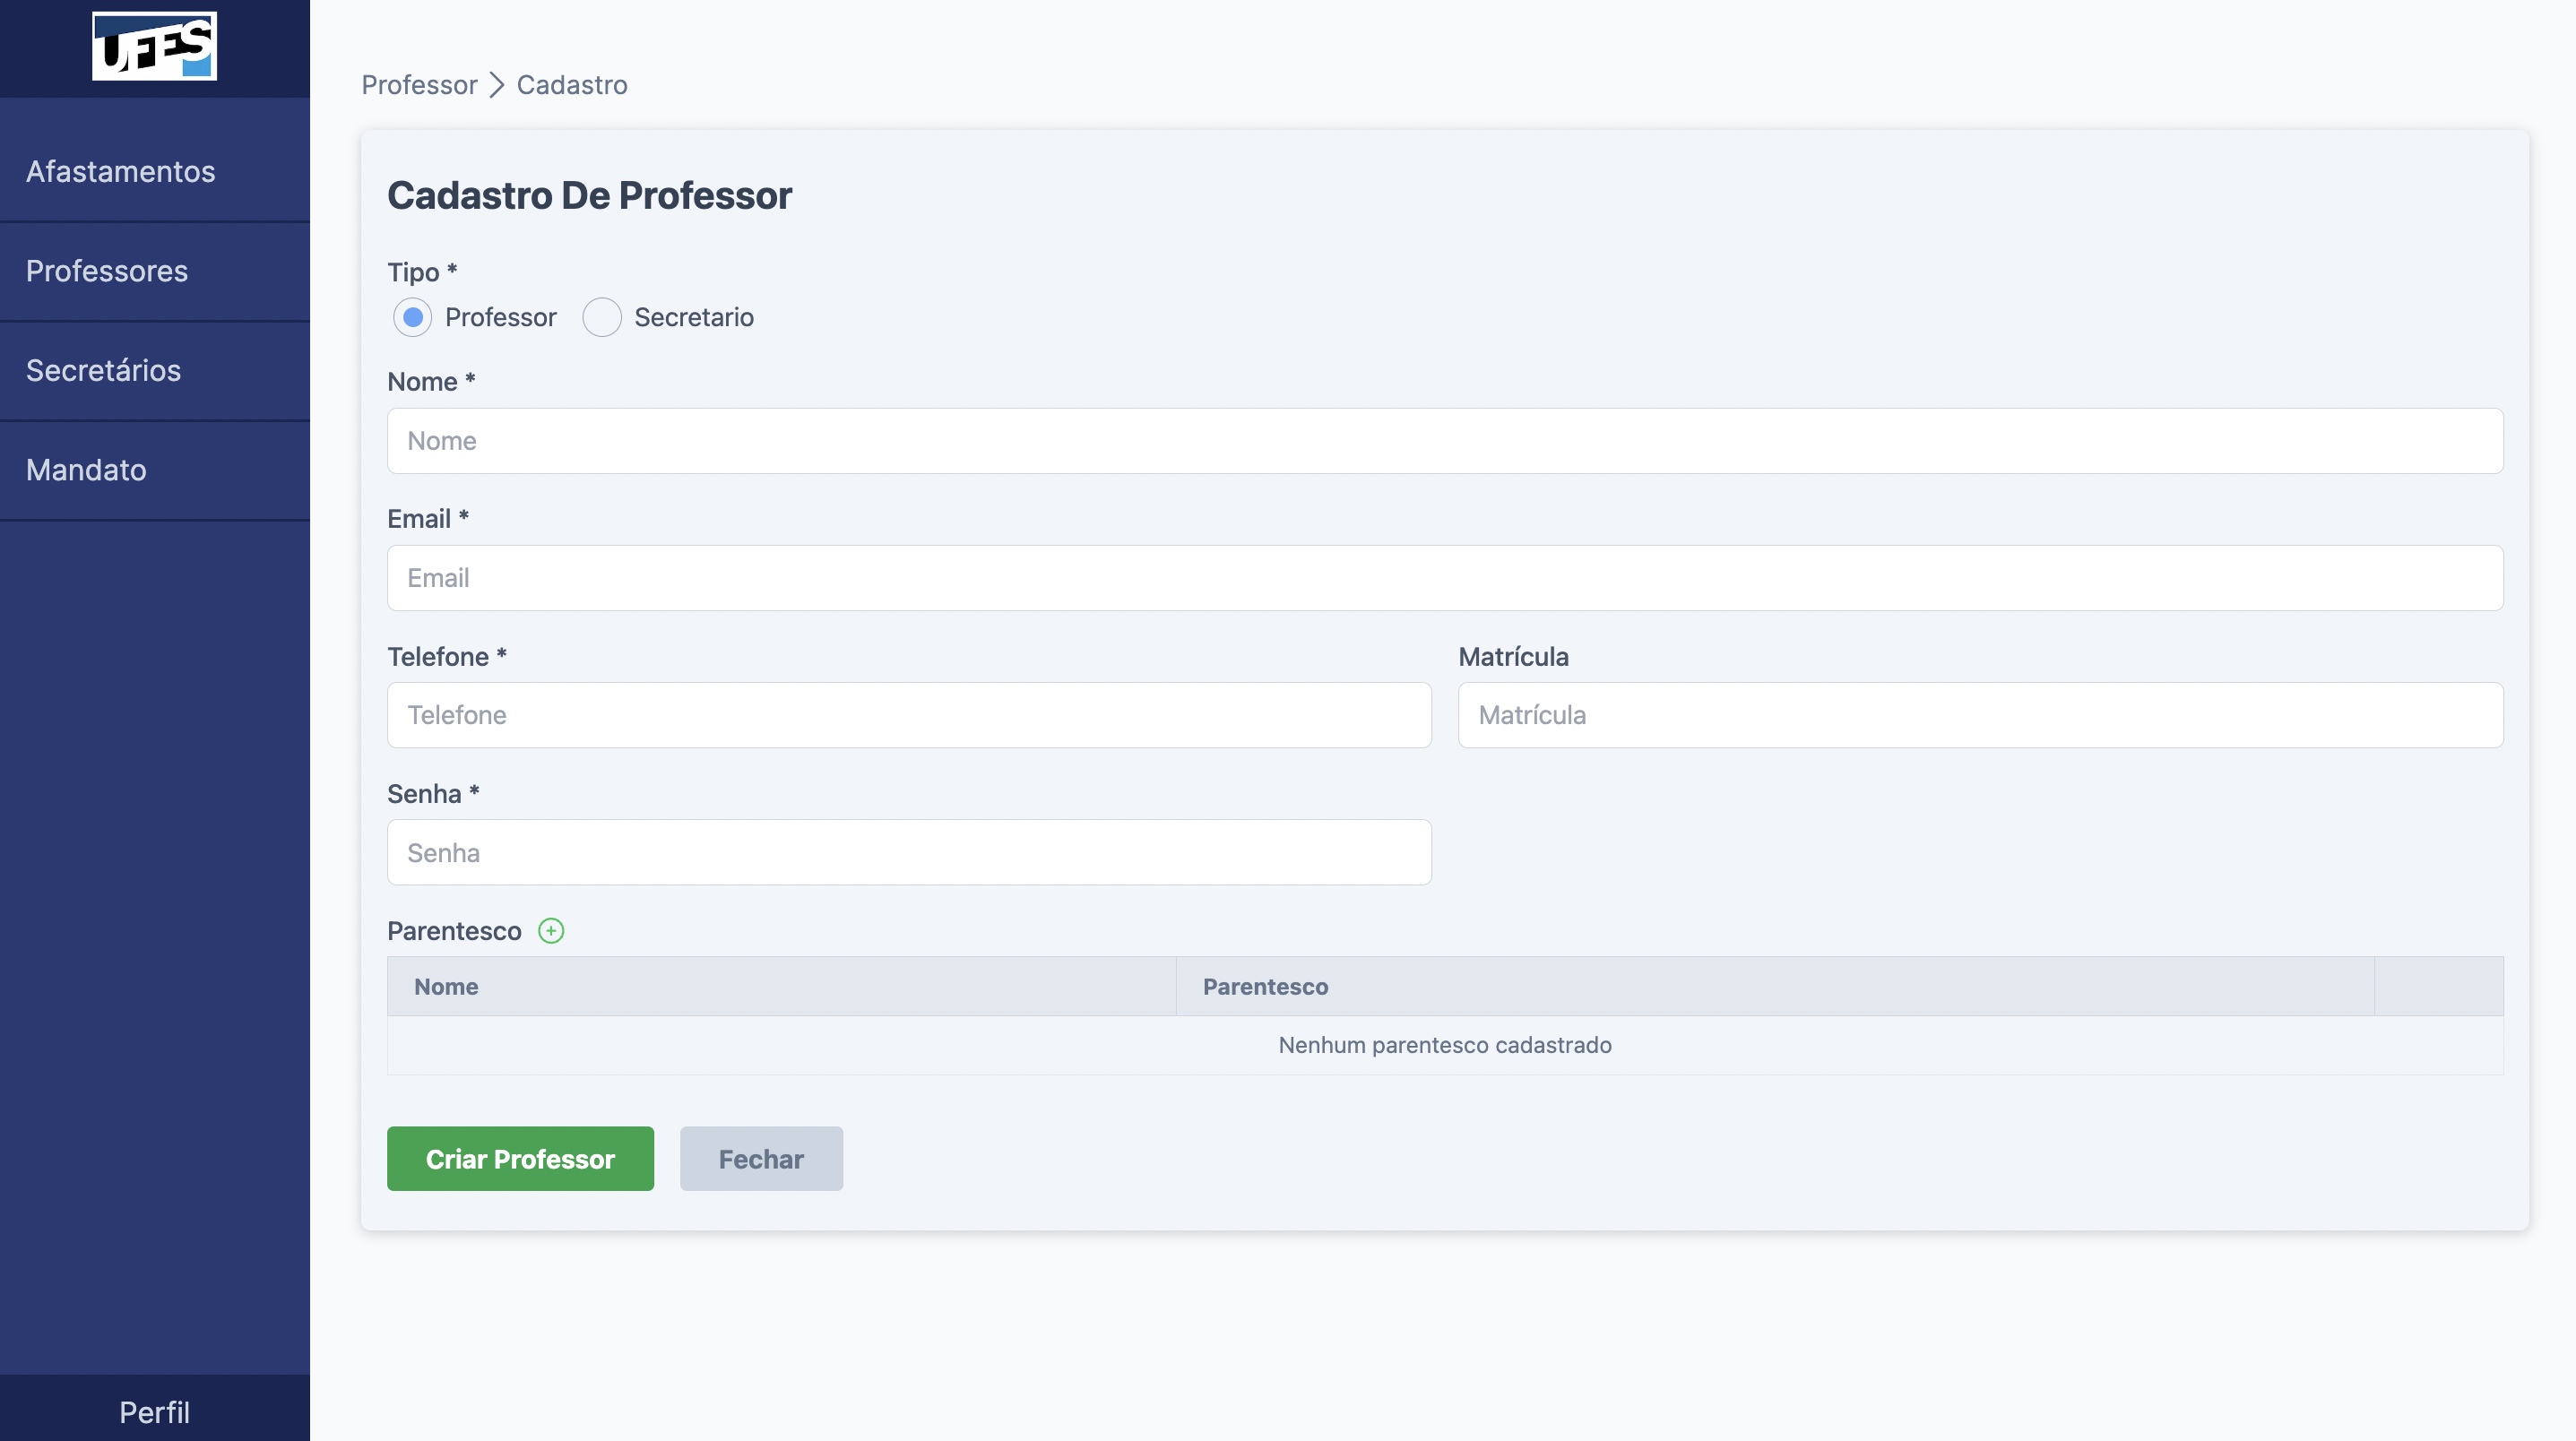
\includegraphics[width=\textwidth]{figuras/prints-app/fig-cadastro-professor.png}
    \caption{Cadastro de Usuários do SCAP.}
    \label{fig-cadastro-professor}
\end{figure}


Caso o usuário a ser criado seja um professor, o secretário pode adicionar parentescos entre professores.
Para isso, deve-se clicar no botão de adição que então abre um modal com um pequeno formulário.
A Figura~\ref{fig-parentesco} apresenta este modal.


\begin{figure}
    \centering
    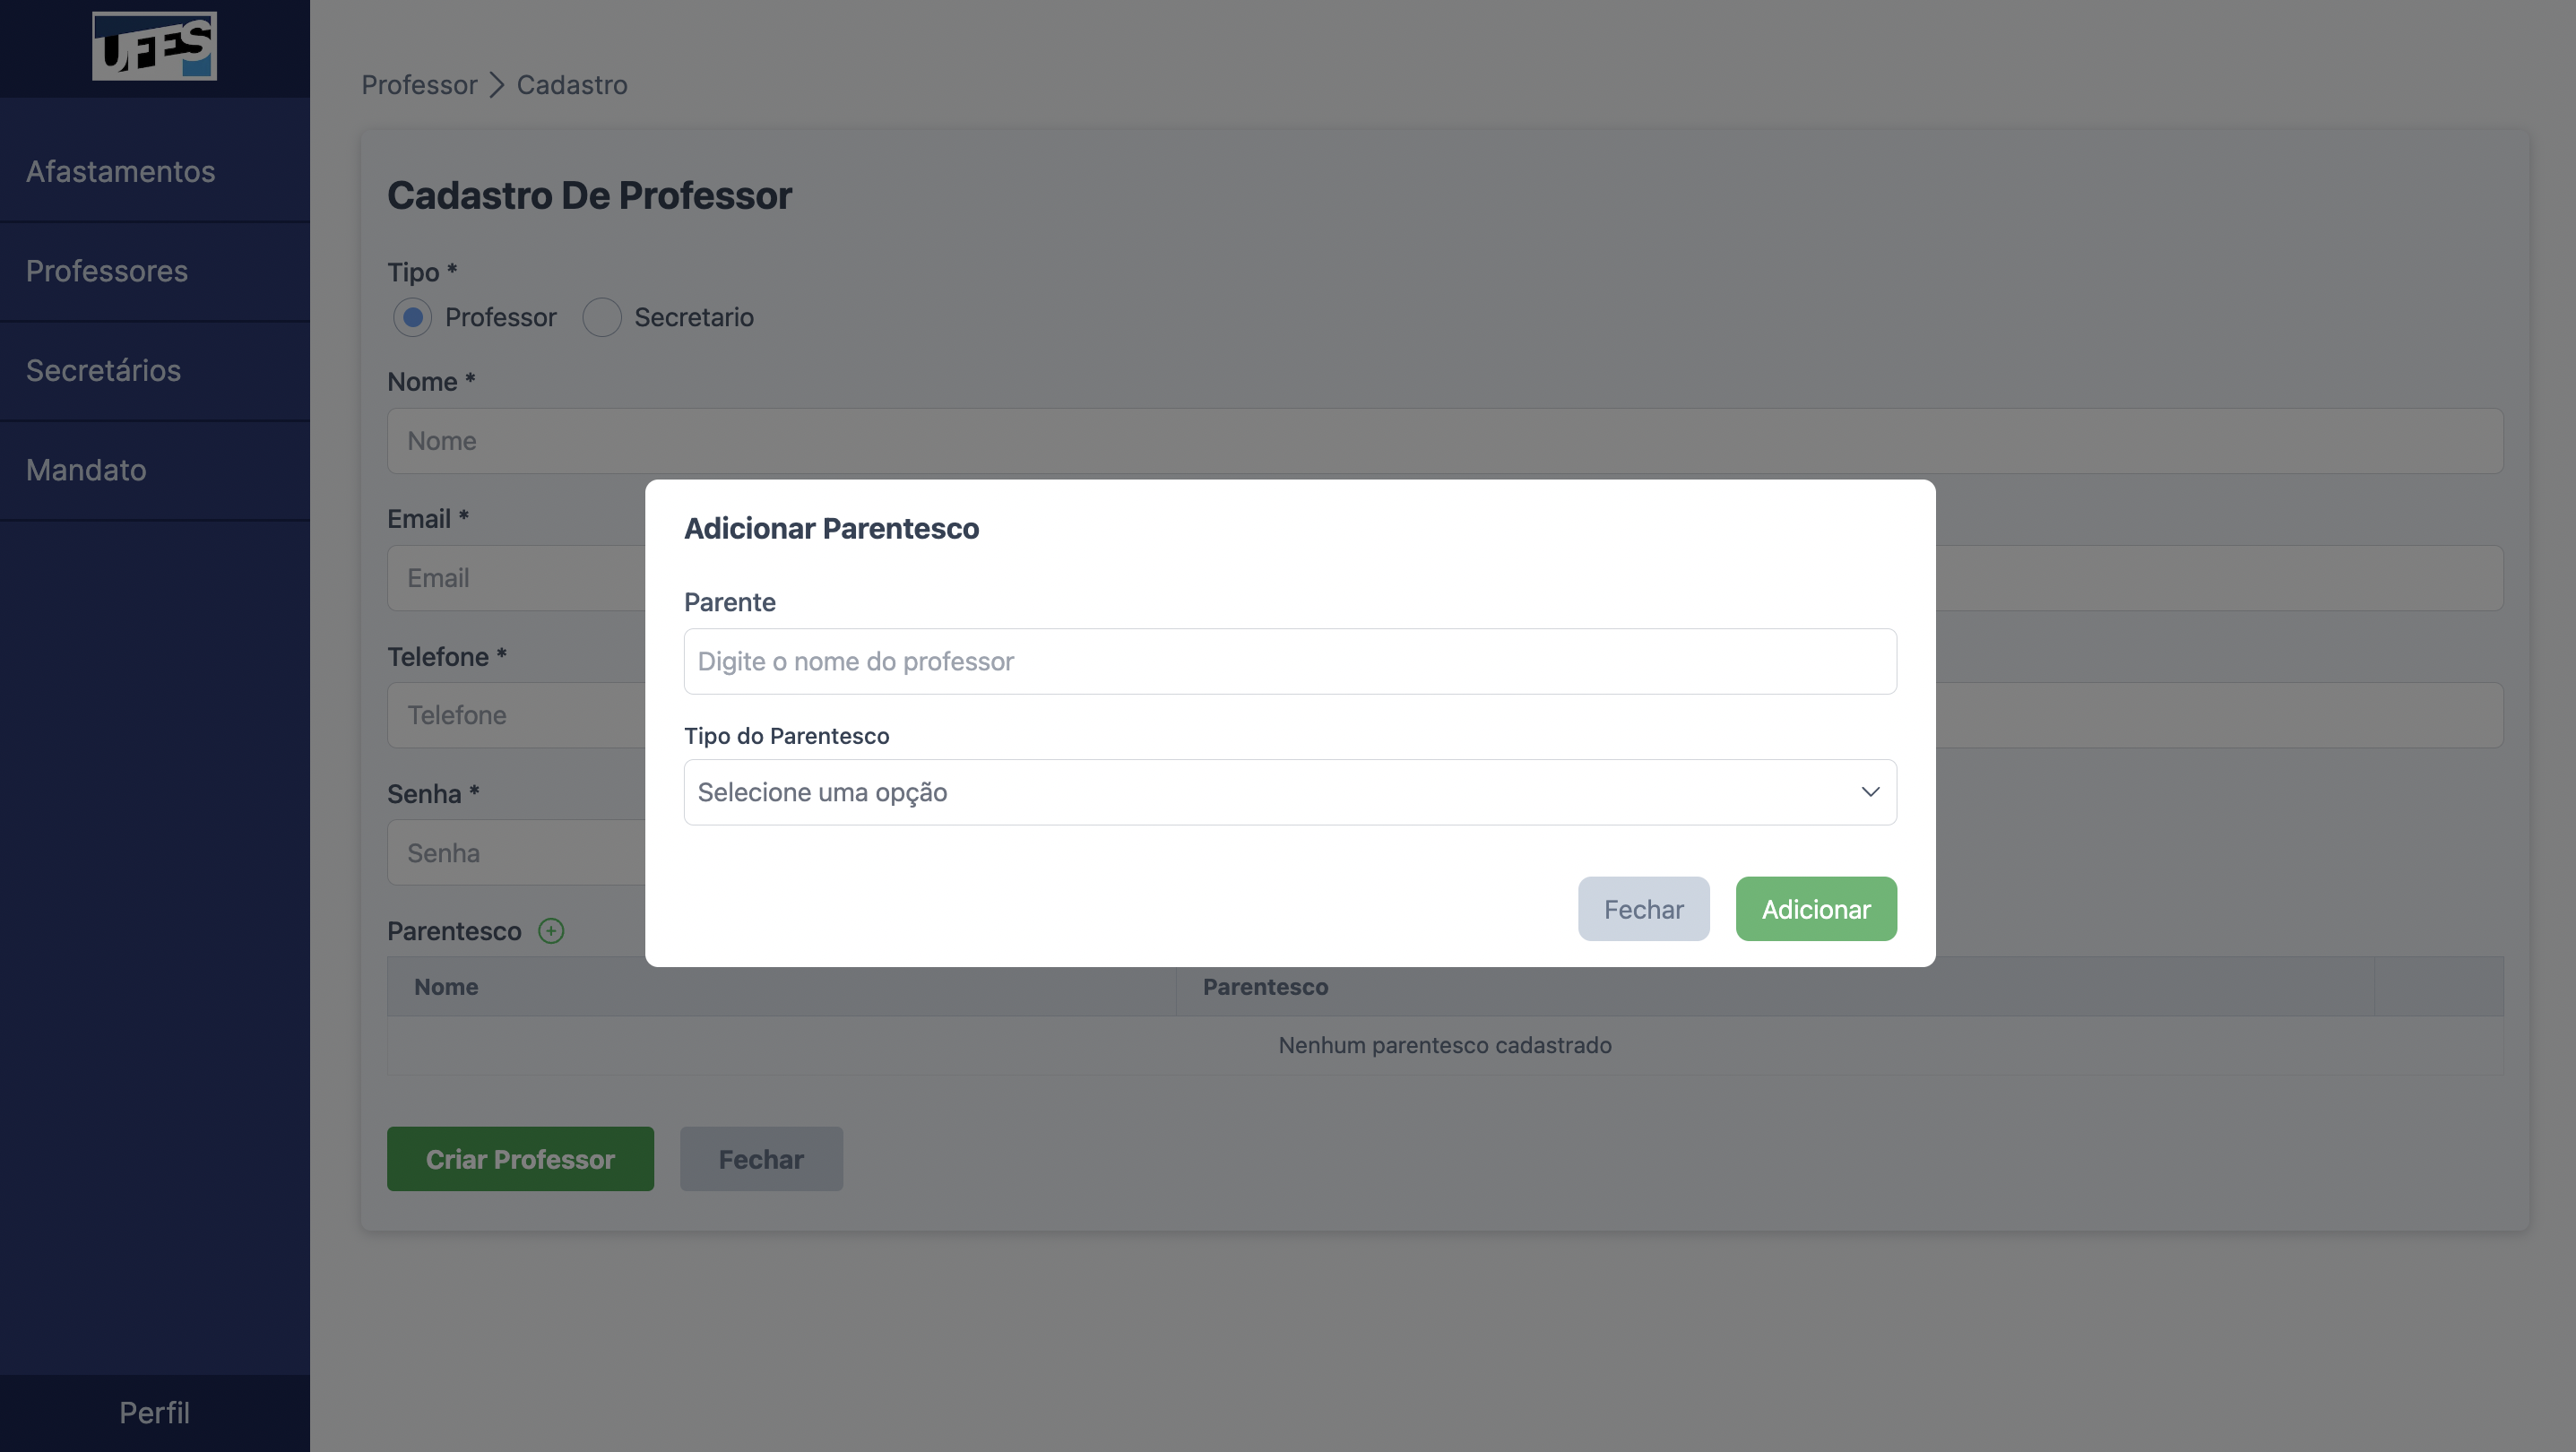
\includegraphics[width=\textwidth]{figuras/prints-app/fig-modal-parentesco.png}
    \caption{Cadastro de Parentesco do SCAP.}
    \label{fig-parentesco}
\end{figure}


O componente de cadastro de usuários é utilizado também para a edição de usuários, assim como foi feito com Afastamentos. A Figura~\ref{fig-editar-professor}
apresenta a página de usuário preenchida com os dados do professor logado no momento. É por essa página também que o usuário pode alterar sua senha ou realizar o \textit{logout} do sistema.

\begin{figure}[h!]
    \centering
    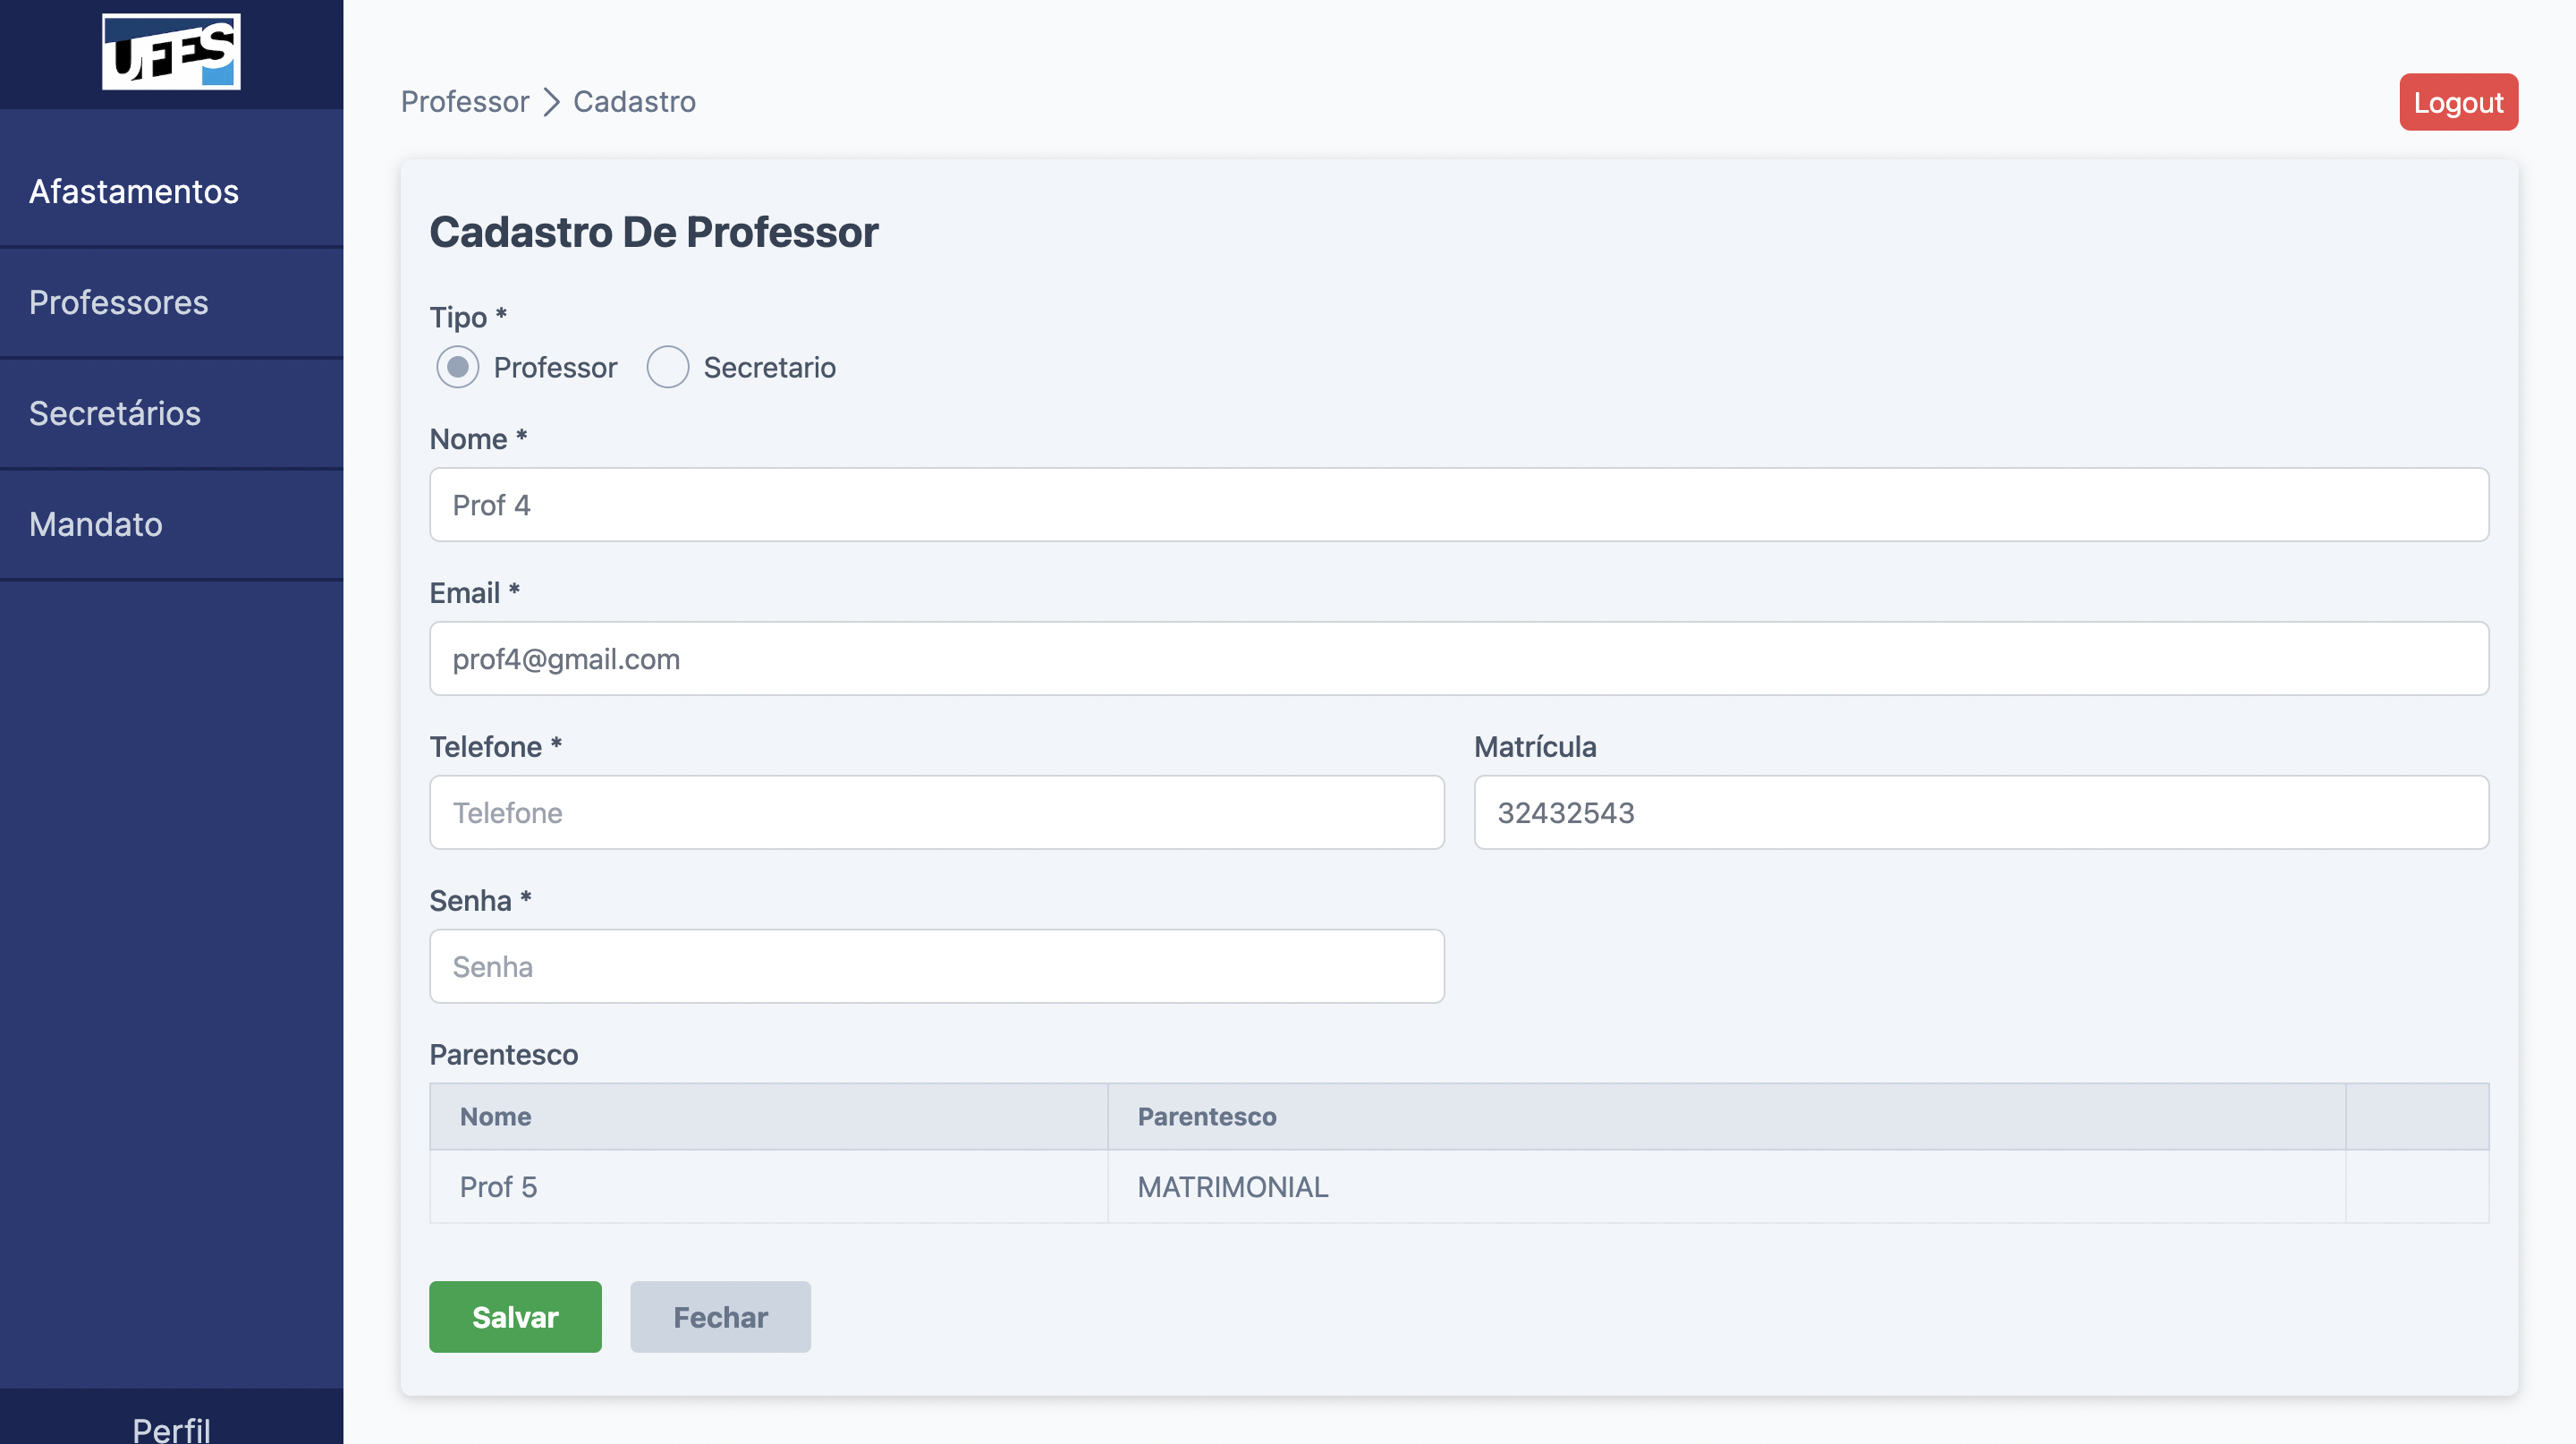
\includegraphics[width=\textwidth]{figuras/prints-app/fig-perfil.png}
    \caption{Edição de Professor do SCAP.}
    \label{fig-editar-professor}
\end{figure}


\subsection{Cadastro de Mandato}
\label{subsec-projeto-cadastro-mandato}

O secretário é responsável por gerenciar os mandatos dos professores, funções que estes exercem
no departamento. A Figura~\ref{fig-mandato} apresenta a tela de cadastro de mandatos do SCAP.
Nela é possível visualizar os mandatos atuais, e para cadastrar um novo mandato deve-se finalizar o anterior.
Para finalizar o mandato basta clicar no botão \textbf{Finalizar Mandato}, caso uma data de fim não seja enviada,
será considerada a data de hoje. Professores também podem visualizar os mandatos atuais. 

\begin{figure}[h!]
    \centering
    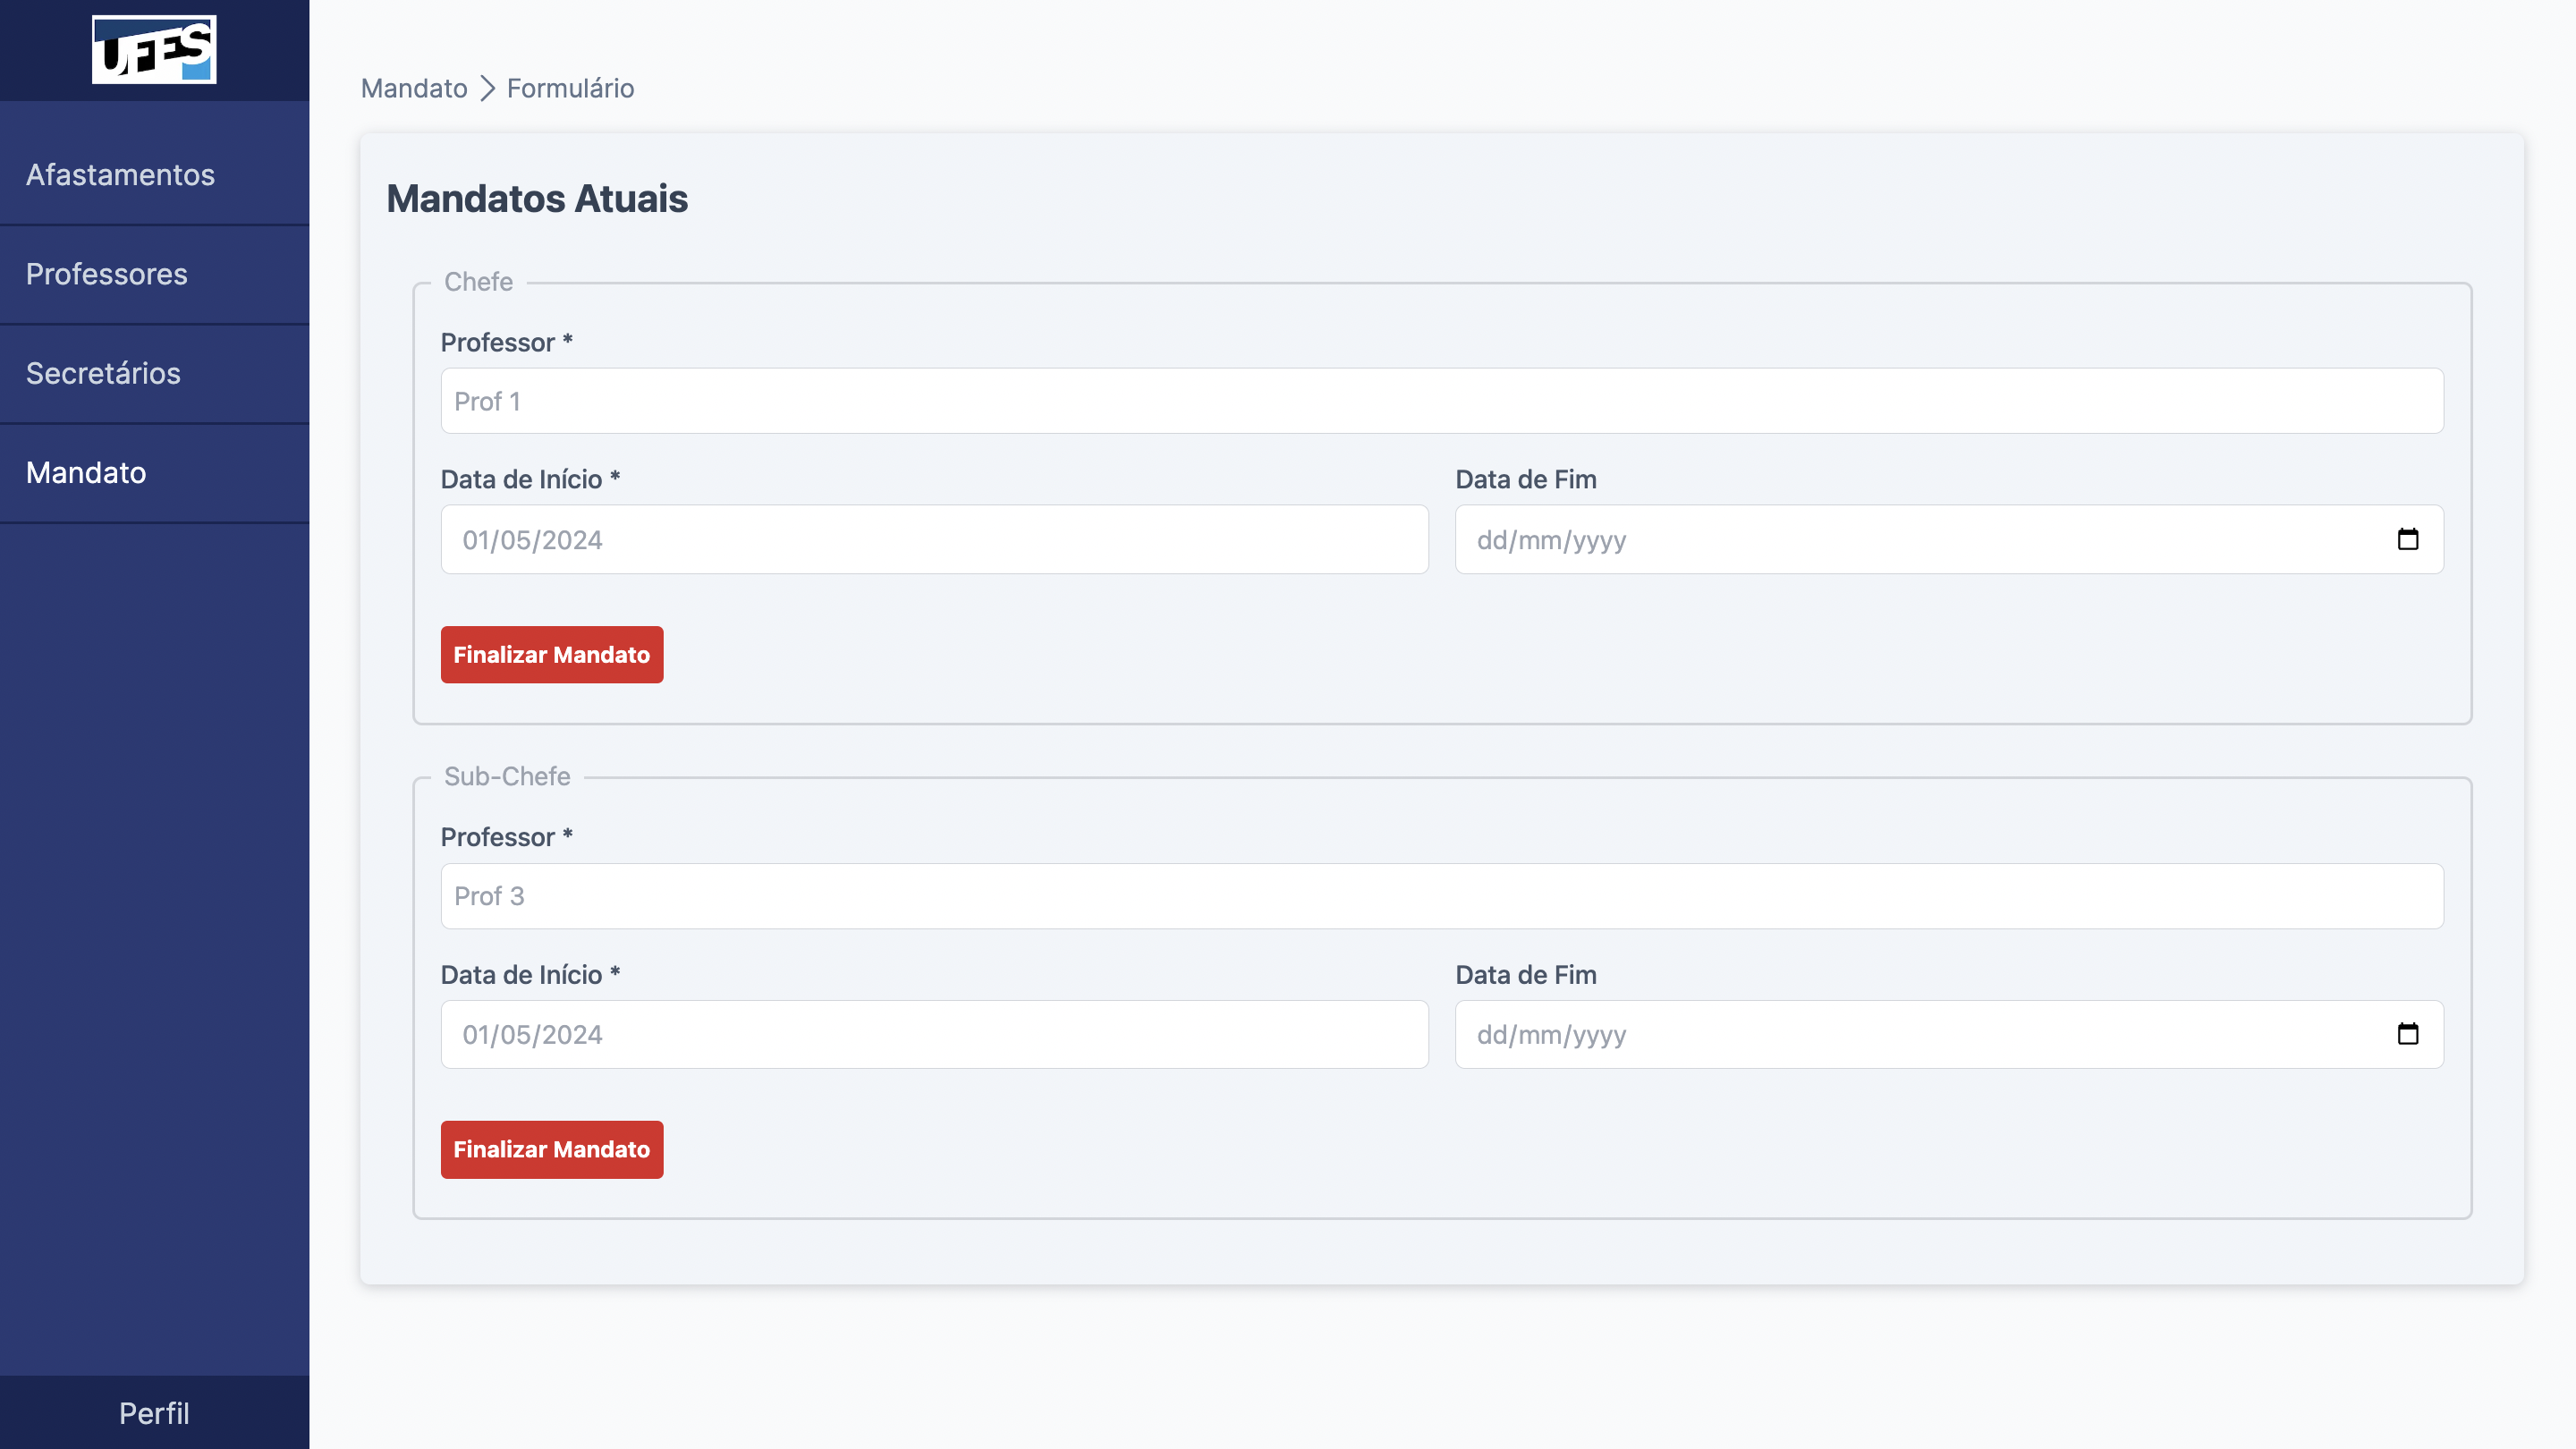
\includegraphics[width=\textwidth]{figuras/prints-app/fig-mandato-visao-secretario.png}
    \caption{Cadastro de Mandatos do SCAP.}
    \label{fig-mandato}
\end{figure}